% !TEX program = xelatex
% =====================================================================
% 《系统工程》专刊「人工智能时代的金融风险管理与系统工程创新」投稿稿
% 题目：信号—状态互补性与多智能体组合的边界条件
%       ——影响因素、边际效应与中国 A 股证据
%
% 说明：本稿为双盲评审稿，正文与元数据均不含作者信息。
% 编译：xelatex main.tex（连续两次）
% =====================================================================
\documentclass[UTF8,a4paper,zihao=-4]{ctexart}

\usepackage{amsmath,amssymb,amsthm,mathtools}
\usepackage{booktabs}
\usepackage{threeparttable}
\usepackage{graphicx}
\usepackage{geometry}
\usepackage{caption}
\usepackage{array}
\usepackage{makecell}
\usepackage{multirow}
\usepackage{enumitem}
\usepackage[hidelinks]{hyperref}
\usepackage{xcolor}
\usepackage{setspace}

\geometry{left=2.6cm,right=2.6cm,top=2.6cm,bottom=2.6cm}
\onehalfspacing
\captionsetup{font=small,labelfont=bf,labelsep=quad}
\setlength{\parindent}{2em}
\setlength{\parskip}{0.15em}

% ---- 定理环境（统一计数器）----
\theoremstyle{plain}
\newtheorem{theorem}{定理}
\newtheorem{proposition}[theorem]{命题}
\newtheorem{lemma}[theorem]{引理}
\newtheorem{corollary}[theorem]{推论}
\theoremstyle{definition}
\newtheorem{assumption}[theorem]{假设}
\newtheorem{definition}[theorem]{定义}
\theoremstyle{remark}
\newtheorem{remark}[theorem]{注}

\newcommand{\E}{\mathbb{E}}
\newcommand{\Var}{\mathrm{Var}}
\newcommand{\Cov}{\mathrm{Cov}}
\newcommand{\Corr}{\mathrm{Corr}}
\newcommand{\Prob}{\mathrm{Pr}}
\newcommand{\R}{\mathbb{R}}
\newcommand{\wtilde}{\tilde{w}}
\newcommand{\bone}{\mathbf{1}}
\newcommand{\bmu}{\boldsymbol{\mu}}
\newcommand{\bSigma}{\boldsymbol{\Sigma}}
\newcommand{\bpi}{\boldsymbol{\pi}}
\newcommand{\Tr}{\mathrm{tr}}

\graphicspath{{../figures/}}

\title{\bfseries 基于多智能体的量化投资策略}
\author{}
\date{}

\begin{document}
\maketitle
\thispagestyle{empty}

\noindent\textbf{摘\quad 要}：多智能体量化投资已成为人工智能在资产管理中的主流实现方式，
其核心是依据市场状态动态合成多个信号（门控组合），但该架构相对静态信号合成的优势缺乏明确条件。本文建立信号—状态互补性框架，
给出门控占优的闭式阈值不等式，并把门控价值解释为信息租金：
只有信号有效性的制度差异（互补性）超过状态信息的获取成本与交易成本，门控才值得做。
基于中国 A 股 868 只证券、247 个月度形成期的点时面板与 2014—2025 年 12 个滚动窗口，
门控组合的年化主动收益为 3.77\%，相对等权的夏普差值为 0.115，
Holm 校正后 $p=0.386$，经济量级明显而统计不显著。
价值集中于高波动与外生冲击年份（冲击年 $+0.173$ 对对照年 $+0.073$），
主要来自二阶风险配置渠道。单边成本每上升 10 个基点使夏普差值下降约 0.015，
盈亏平衡成本约 92 个基点；制度状态数在 3 处呈内点最优。
结论对制度定义与推断设定敏感。

\vspace{0.4em}
\noindent\textbf{关键词}：多智能体组合；信号—状态互补性；信息租金；制度切换；估计误差；交易成本；金融风险管理

\vspace{0.3em}
\noindent\textbf{中图分类号}：F830.59；F224.0

\vspace{0.8em}
{\raggedright\small
\noindent\textbf{Multi-Agent Quantitative Investment Strategies}\par

\vspace{0.3em}
\noindent\textbf{Abstract}: Gated multi-agent portfolios have become a default architecture
in research at the intersection of artificial intelligence and quantitative investment,
yet their advantage over static combination lacks explicit conditions. This paper develops
a signal--state complementarity framework, derives a closed-form threshold inequality for
gating dominance, and interprets the value of gating as an information rent: gating pays
only when the regime-dependence of signal effectiveness exceeds the cost of acquiring
regime information and the cost of trading. Using a point-in-time monthly panel of 868
Chinese A-share stocks over 247 formation months with 12 annual rolling windows from 2014
to 2025, we
find that the gated portfolio earns an annualized active return of 3.77\% and a Sharpe
difference of 0.115 against equal weighting, which is economically sizable but
statistically insignificant after Holm adjustment ($p=0.386$); its relative value
concentrates in high-volatility years and in years of exogenous shocks (+0.173 versus
+0.073 in other years), and originates mainly from the second-order risk-allocation
channel. A 10-basis-point increase in the one-way
transaction cost lowers the Sharpe difference by about 0.015, with a break-even cost of
roughly 92 basis points, and the number of regimes exhibits an interior optimum at
three. The conclusions are sensitive to the regime definition and the bootstrap block
length, and complementarity is not identifiable in a narrow cross-section. The
threshold inequality turns the question of whether gating is worthwhile into a decision
problem that can be independently recomputed.
\vspace{0.3em}
\noindent\textbf{Keywords}: multi-agent portfolio; signal--state complementarity;
information rent; regime switching; estimation error; transaction cost;
financial risk management\par
}

\setcounter{page}{1}

\section{引言}

人工智能正在改变金融风险的识别、计量与防控方式，也在改变资产管理的实现路径。
大模型、图神经网络与强化学习等方法与复杂网络、多主体仿真等系统工程方法相互融合，
为市场风险与流动性风险的计量提供了新的工具\cite{hong2021,suzhi2017,wangfang2020}。
在这一背景下，多智能体量化投资的核心任务是把多个预测信号合成为可执行的组合。
机构投资者与量化管理人通常同时维护动量、反转、低波动、换手、估值与情绪等多个信号，
合成方式有两种。
静态合成以固定权重平均各信号；状态自适应合成（本文称门控组合）依据市场状态、
各信号近期表现与风险暴露动态调整信号权重。
随着多智能体系统与深度强化学习组合管理框架的流行\cite{jiang2017,liu2020,li2024}，
门控组合已成为多智能体量化投资中的默认架构。这一架构隐含地假设状态自适应优于静态合成，
但该假设缺乏明确的经济学条件。已有研究更多关注架构设计本身——增加智能体数量、
引入记忆机制、构造更复杂的门控网络——较少回答三个更基本的问题：

其一，条件问题：在什么条件下，状态自适应门控能带来扣除交易成本后的可测超额收益？
其二，来源问题：门控收益来自对不同状态下信号收益水平的预测（收益择时），
还是来自对不同状态下信号风险结构的配置（风险配置）？
其三，识别问题：给定样本的时间长度与横截面宽度，这一收益能否被统计地识别？

三个问题的答案决定风险管理资源的配置方向。若门控收益来自收益择时，
其识别依赖时间维度，在市场结构变化时容易失效；若收益来自风险配置，
低波动与风险平价等更简单的风险结构策略可能是更高效的实现方式。
对资产管理机构而言，判断门控是否值得做决定了模型容量、数据采购与交易系统的投入；
对监管者而言，人工智能投顾与量化资管中的「自适应」「智能」等业绩宣称需要可复核的判定标准。

本文研究多智能体量化投资策略的价值边界。核心判断是：复杂门控并不必然优于简单平均。
门控只有在信号的预测能力随市场状态出现足够大的差异（互补性），
且这一差异超过状态信息的获取成本与交易成本时才有价值；
否则，复杂的门控只是在为无法利用的状态差异支付估计与交易成本。
这一判断把「何时使用门控」从架构偏好转变为成本收益比较，
并把门控收益的性质界定为信息租金：它与信息经济学中「信息有价、
但价格不能长期高于获取成本」的逻辑同源\cite{grossman1980}。

在长仓满仓这一标准约束下（$w_t\in\{w\in\R^N_+:\bone^\top w=1\}$），组合收益可分解为
\begin{equation}
r_{p,t+1}=w_t^\top r_{t+1}=r_{ew,t+1}+\wtilde w_t^\top r_{t+1},
\qquad \wtilde w_t=w_t-w^{ew},\quad w^{ew}=\bone/N,
\label{eq:intro-decomp}
\end{equation}
其中 $r_{ew,t+1}$ 为等权组合收益。由 $\bone^\top\wtilde w_t=0$，组合的相对表现完全由
主动权重 $\wtilde w_t$ 决定，而 $r_{ew,t+1}$ 与决策无关。该分解的直接含义是：
以绝对收益为训练目标时，目标中与决策无关的基准项不提供梯度信息，
唯一较强的梯度来自换手惩罚，优化因此收敛到「不交易」这一平凡解。
命题 \ref{prop:degeneracy} 给出退化发生的精确参数条件。

该诊断有直接的实证对应物。在一个以十只美国 ETF 为样本、以绝对收益为目标的多智能体门控模型中，
平均换手率仅为 0.0029，与静态持有水平相当；组合夏普比率（0.940）与等权基准（0.941）
几乎一致，配对检验的 95\% 区间跨越零、Holm 校正后 $p=1.000$。
这一「自适应门控」实际上退化为静态等权，其零结果不是实验失败，而是目标函数设计的产物。
该现象影响文献中一类结论的可信度：在满仓长仓约束下报告「自适应优势」的研究，
若不同时报告组合相对基准的主动暴露，读者无法区分机制奏效与机制退化。

把训练目标改为主动收益即可消除退化：式 \eqref{eq:intro-decomp} 中被消去的基准项
不再主导梯度，门控具备识别信号—状态互补性的条件。

本文建立信号—状态互补性框架。门控相对最优静态合成的价值等于互补性收益
减去估计误差成本与换手成本，门控占优的充要条件是一个具有闭式解的阈值不等式
\begin{equation}
\hat\Gamma>\Theta+2\lambda\kappa\,\mathcal{C}(\hat g),
\label{eq:intro-threshold}
\end{equation}
其中 $\hat\Gamma$ 为互补性统计量，$\Theta$ 为估计噪声底线，$\kappa$ 为单边交易成本。
互补性可分解为一阶（条件均值）与二阶（条件波动与相关结构）两条渠道，
两者的噪声底线分别以 $O(1/T)$ 与 $O(1/(NT))$ 收敛；制度的马尔可夫持续性通过几何乘数
放大门控的信息价值；在容量约束下净价值关于制度数呈单峰，最优制度数内点存在；
横截面宽度不足时，互补性在统计上不可识别。

实证部分使用 2006 年 1 月至 2026 年 7 月中国 A 股月度点时面板（868 只证券、
247 个月度形成期、月均进入股票池 438 只），以 2014 年至 2025 年 12 个年度滚动窗口
进行样本外检验。

门控组合的表现与来源。门控组合的年化主动收益为 3.77\%，主动信息比率为 0.80，
相对等权的夏普差值为 $+0.115$（95\% 区间 $[-0.006,0.225]$，Holm 校正后 $p=0.386$），
经济量级明显而统计上不显著。按定理 \ref{thm:threshold}，
这一结果与两条渠道的互补性检验互相印证：一阶与二阶互补性统计量分别为
$3.93\times10^{-4}$ 与 $6.34\times10^{-4}$，对应噪声底线 $4.17\times10^{-4}$ 与
$6.87\times10^{-4}$，$p$ 值为 0.060 与 0.065。安慰剂检验把门控主动收益由 3.77\% 压至
0.004\%，说明收益依赖制度信息；而允许使用制度内真实条件期望收益的 Oracle 门控
（夏普 0.562）未跑赢静态合成（0.546），说明可利用的一阶互补性有限。
门控收益主要来自二阶风险配置渠道。

影响因素。门控的相对价值不恒定。年度市场波动率最低的三分之一年份，
相对等权的夏普差值平均为 $+0.006$；最高的三分之一年份升至 $+0.189$。
横截面离散度与制度切换次数呈现同向的分组特征，而市场涨跌方向与差值的关系微弱
（秩相关 $-0.049$）。门控的价值来自市场状态的分化程度，而非市场方向。
外生冲击进一步放大了这一分布：把 2015 年股市异常波动、2016 年熔断机制实施、
2018 年中美贸易摩擦、2020 年新冠疫情、2022 年俄乌冲突与疫情封控五个年份
作为冲击年（事件时间由外部事件日历决定），冲击年的夏普差值平均为 $+0.173$，
其余年份为 $+0.073$，差值为 $+0.100$（95\% 区间 $[-0.081,0.276]$）。
冲击年的市场波动率更高（0.291 对 0.202），制度切换次数与其余年份接近（3.20 对 3.29），
门控价值与状态分化的幅度相关，而非切换的频率。

边际效应。单边交易成本每上升 10 个基点，相对等权的夏普差值下降约 0.015
（$p<0.001$），盈亏平衡成本约为 92 个基点。制度状态数呈内点最优：
由 2 增至 3 使夏普差值提高 0.079，由 3 增至 4 转为下降 0.014。
训练窗长度没有单调效应（斜率 $-0.006\,3$/年，$p=0.617$）。

稳健性与边界。门控优势在 2020 年后的子样本中由 $+0.180$ 收窄至 $+0.049$；
四种制度定义下夏普跨度约 0.16，与门控的整体优势同量级；
阈值检验的显著性依赖自助区块长度，3--6 个月时至少一条渠道显著，
12--24 个月时两条渠道均不显著；在 10 只美国 ETF 的窄横截面上互补性不可识别。

相对于以绝对收益为目标、以架构复杂度为创新点的那类多智能体研究，
本文的增量体现在三个方面。理论上，本文把门控价值分解为互补性收益、
估计误差成本与换手成本，给出门控占优的充要条件、两条渠道的分离、
持续性的乘数效应与容量约束下的最优制度数，并把门控收益界定为信息租金，
把「预测组合之谜」解释为该框架的特例。方法上，本文识别了满仓长仓约束下
绝对收益目标的退化问题并给出主动收益的修正，构造了可自校准的互补性阈值检验、
渠道识别检验与 Oracle 上界检验，并用外生冲击年份构成识别设计。
实证上，本文在中国 A 股市场提供严格滚动样本外检验，
用三类独立检验交叉验证门控收益的来源与量级，并给出多智能体策略价值对交易成本、
制度数与训练窗长度的边际效应估计。

余下部分安排：第 \ref{sec:lit} 节综述相关文献；第 \ref{sec:framework} 节给出分析框架；
第 \ref{sec:design} 节说明研究设计；第 \ref{sec:factors} 节报告影响因素；
第 \ref{sec:marginal} 节报告边际效应；第 \ref{sec:robust} 节检验稳健性；
第 \ref{sec:policy} 节讨论政策含义；第 \ref{sec:conclusion} 节总结。

\section{文献综述}
\label{sec:lit}

多智能体与强化学习组合管理。把组合决策表述为连续控制问题的研究由深度强化学习
框架系统化\cite{jiang2017}，此后 FinRL 等开源环境把市场模拟、算法与回测流程整合为
统一实验平台\cite{liu2020}，多策略协调研究进一步在收益策略与风险策略之间引入
动态协调机制\cite{li2024}。算法层面的基础工作确立了确定性策略梯度与自举式价值估计的
可行性\cite{mnih2015,lillicrap2016,sutton2018}，金融场景的系统评述与端到端组合优化实现
可分别参见 \cite{charpentier2023} 与 \cite{cong2021}。这类研究的共同设定是：
以历史数据训练一个状态到权重的映射，并用样本外表现作为评价标准。
其目标函数通常是绝对财富或绝对收益，在满仓长仓约束下该目标存在结构性退化——
与决策无关的基准收益项主导梯度，剩余梯度主要来自换手惩罚，机制收敛于静态等权。
本文分离出这一退化并给出主动收益的修正方案，使自适应机制具备识别互补性的条件
（命题 \ref{prop:degeneracy}）。

状态自适应资产配置。Hamilton 的马尔可夫状态切换模型为刻画收益分布的制度变化
提供了基础工具\cite{hamilton1989}，Guidolin 和 Timmermann 将其用于资产配置，
发现状态切换改善样本外表现\cite{guidolin2007}。这一传统隐含「状态可识别即有配置价值」
的判断。本文证明该判断不充分：即使状态被完美识别，若信号有效性不随状态变化
（$\Gamma=0$），门控的价值仍为零（推论 \ref{cor:identification}）。
状态识别的价值取决于互补性与持续性两个条件，本文将两者写成可估计的对象，
为「何时使用状态切换模型」提供了可计算的判据。

预测组合与「组合之谜」。预测组合文献记录了一个稳健事实：
简单平均预测经常打败样本内最优的估计权重组合\cite{timmermann2006}；
相关经典结果包括协方差矩阵收缩\cite{ledoit2004}与等权组合的样本外稳健性
\cite{demiguel2009}。既有解释多归于「估计误差」，但缺少可计算的临界值。
本文给出的阈值不等式补上这一环：$\Theta$ 就是「组合之谜」的临界线，
$\hat\Gamma<\Theta$ 时估计最优权重不如简单平均。渠道分解进一步说明，
二阶矩比一阶矩更容易估计，以风险配置为主的合成本质上比以收益择时为主的合成
更容易获得稳健收益。这为「简单策略为何难以被超越」提供了一个新的解释维度。

互补性的第一个来源：信息成本与注意力配置。门控价值来自互补性，
而互补性需要经济学来源。Grossman 和 Stiglitz 指出，若价格已充分反映信息，
收集信息便无利可图，市场因此不可能完全有效\cite{grossman1980}；
Sims 的理性疏忽理论说明，决策者处理信息的能力受有限信道容量约束，
会把注意力配置给成本低、精度高的信息源\cite{sims2003}；
DellaVigna 和 Pollet 的证据显示注意力不足会延迟信息进入价格\cite{dellavigna2009}。
这条线索对本文有两个推论。其一，同一信号在不同市场状态下的信息含量不同：
状态决定了哪些公开信息与收益更相关，信号的预测精度随状态变化，互补性因此为正。
其二，状态信息本身有价格：估计条件信息系数需要按状态切分样本，
每格的估计精度随样本量下降，这一估计误差成本正是本文阈值中的 $\Theta$。

互补性的第二个来源：行为偏差的状态依赖。Odean 记录的处置效应使投资者
过早卖出盈利、过久持有亏损\cite{odean1998}；Barber 和 Odean 记录过度自信
提高交易频率并降低净收益\cite{barberodean2001}；Hong 和 Stein 的统一理论说明，
信息在不同投资者群体间的逐步扩散可以同时产生动量和反转\cite{hongstein1999}。
这类偏差的强度随市场状态变化，上涨行情中的过度自信与下跌行情中的处置效应更为突出，
以动量和反转为基础构造的信号，其有效性因此带有状态依赖。
本文的专家信号集合正由这类价量信号构成，互补性因此不是设定假设，而是可估计的对象。

渠道差异的理论对应：有限套利。「一阶互补性有限、二阶互补性为主」
这一发现的对应理论是有限套利与信息的估计成本差异。基于收益水平（一阶矩）的套利
需要承担基本面风险与噪声交易者风险，在资金约束下难以充分实施\cite{shleifer1997}；
而波动率与相关性（二阶矩）可以从公开价格序列以较低成本估计。
理性疏忽的预测正是把注意力配置给后者，本文的渠道分解为该预测提供了
横截面资产配置场景下的证据。

机器学习资产定价与稳健性检验。机器学习在收益预测中的应用已成体系。
Gu 等在美国股票横截面上比较十三类模型，报告树集成与神经网络的样本外 $R^2$
相对线性模型提升逾一倍\cite{gu2020}，并在自编码器与深度学习方法上做了拓展
\cite{gu2021,chen2024}。与之并行的是对多重检验的批评：Harvey 等要求新因子满足
更高的 $t$ 值门槛\cite{harvey2016}，Feng 等在给定已有因子的条件下检验新增因子的
定价信息\cite{feng2020}，Kozak 等指出高维因子的定价信息由少数主成分承载
\cite{kozak2020}，Kelly 等讨论模型复杂度与样本量的匹配关系\cite{kelly2024,kelly2023}。
中国市场的机器学习量化投资与文本情绪信号已有系统证据\cite{libin2019,jiang2021,shen2019}，
金融机器学习的方法论综述则强调回测过拟合、信息泄漏与前视偏差的风险
\cite{lopezdeprado2018}。本文属于该传统的稳健性检验分支，检验对象是模型组合机制本身：
本文要求报告「自适应优势」的研究同时给出主动暴露、互补性与噪声底线的对比、
以及渠道分别检验。三组诊断量的计算成本低，作用是把机制奏效与机制退化区分开。

人工智能在金融系统中的治理含义。机器学习在信贷、支付与投顾环节的渗透
使可解释性与公平性成为监管议题。Fuster 等发现算法定价在降低成本的同时
对部分群体产生差异化影响\cite{fuster2022}；基础模型的能力与风险综述指出，
模型规模扩张不自动带来可靠性\cite{bommasani2021}；中央银行视角的研究关注
机器学习在监管科技中的应用与边界\cite{chakraborty2017,bis2024aer}。
本文的阈值不等式与三组诊断量回应这一议题：它把「人工智能组合是否真的更优」
转化为可在同一数据集上独立复算的问题，为算法审计提供可执行的判据。

表 \ref{tab:lit-map} 归纳本文与各组文献的差异边际。

\begin{table}[htbp]
\centering
\caption{文献群、缺口与本文增量}
\label{tab:lit-map}
\begin{threeparttable}
\footnotesize
\begin{tabular}{p{2.5cm}p{5.4cm}p{5.3cm}}
\toprule
文献群 & 已有贡献与留下的缺口 & 本文增量 \\
\midrule
多智能体与强化学习组合管理 & 建立了状态到权重的映射框架；
目标函数多为绝对收益，未识别退化解 & 分离出满仓约束下的退化机制，
给出主动收益修正（命题 \ref{prop:degeneracy}） \\
状态自适应资产配置 & 证明状态切换可改善配置；
默认「状态可识别即有配置价值」 & 给出门控价值的充要条件，
说明识别状态不等于有价值（推论 \ref{cor:identification}） \\
预测组合与组合之谜 & 记录简单平均的稳健优势，
以估计误差笼统解释 & 给出临界值的闭式解与比较静态，
把经验规律变为可复算判据（定理 \ref{thm:threshold}） \\
信息经济学与行为金融 & 说明信息的成本、注意力的稀缺与偏差的状态依赖；
未落到多信号合成的决策 & 把互补性追溯到信息成本与行为偏差，
并以渠道分解检验其可识别性（定理 \ref{thm:channels}） \\
机器学习资产定价与稳健性 & 建立了预测与多重检验的规范；
检验对象是单一模型 & 把稳健性检验对象扩展到组合机制，
提出三个低成本诊断量 \\
人工智能金融治理 & 关注可解释性、公平性与监管科技的边界；
缺少可操作的判定程序 & 提供可在同一数据集复算的阈值判据，
把审计要求落为具体计算 \\
\bottomrule
\end{tabular}
\end{threeparttable}
\end{table}

\section{分析框架}
\label{sec:framework}

设资产 $i=1,\dots,N$，专家（信号）$k=1,\dots,K$，市场制度 $s=1,\dots,S$，
样本期数 $T$。制度过程 $\{s_t\}$ 为一阶马尔可夫链，转移矩阵 $P=(p_{sl})$，
平稳分布 $\bpi=(\pi_1,\dots,\pi_S)$。资产条件期望收益与协方差记为
$\bmu_s=\E[r_{t+1}\mid s_t=s]$、$\bSigma_s=\Var(r_{t+1}\mid s_t=s)$。
组合空间为长仓满仓单纯形，基准取等权 $w^{ew}=\bone/N$，
主动权重 $\wtilde w_t=w_t-w^{ew}$。

\begin{lemma}[基准恒等式]
\label{lem:identity}
对任意长仓满仓组合 $w_t$，$r_{p,t+1}-r_{ew,t+1}=\wtilde w_t^\top r_{t+1}$。
\end{lemma}

证明由 $\bone^\top w_t=\bone^\top w^{ew}=1$ 直接得到，不依赖任何分布假设。
该恒等式说明满仓长仓组合的相对表现完全由主动权重决定，与市场整体涨跌无关。
它同时意味着，绝对收益目标中与决策无关的 $r_{ew}$ 项无法为权重选择提供信息，
这是退化命题的起点。

专家 $k$ 由特征向量 $x_{i,t}$ 产生截面打分 $\theta_{k,i,t}=\phi_k(x_{i,t})$，
并通过带温度参数 $\tau_k>0$ 的 softmax 映射为组合权重
\begin{equation}
a_{k,i,t}=\frac{\exp(\theta_{k,i,t}/\tau_k)}{\sum_{j=1}^N\exp(\theta_{k,j,t}/\tau_k)} .
\label{eq:softmax-expert}
\end{equation}
$\tau_k\to\infty$ 时专家趋向等权，$\tau_k\to0$ 时专家集中持有打分最高的少数资产。
门控权重 $g_t\in\Delta^{K-1}$ 由状态、专家置信度、专家风险与近期表现决定，
组合权重为 $w_t=\sum_k g_{k,t}a_{k,t}$。

\begin{assumption}[制度切换因子结构]
\label{ass:factor}
资产条件期望收益可表示为 $\bmu_s=\sum_{k}b_{k,s}\tilde{\boldsymbol\theta}_{k}
+\varepsilon_s$，其中 $b_{k,s}$ 为专家 $k$ 在制度 $s$ 中的条件信息系数，
$\tilde{\boldsymbol\theta}_k$ 为去均值后的打分向量，
且 $\E[\varepsilon_s\mid\mathcal{F}_t]=0$、$\E[\tilde{\boldsymbol\theta}_k^\top\varepsilon_s]=0$。
\end{assumption}

假设 \ref{ass:factor} 把专家的预测能力按制度分解，并允许不同制度下的系数 $b_{k,s}$ 不同。
这是「状态自适应」在数据中的对应物。

\begin{definition}[信号—状态互补性]
\begin{equation}
\Gamma_k=\sum_{s=1}^S\pi_s\big(b_{k,s}-\bar b_k\big)^2,
\qquad \bar b_k=\sum_{s=1}^S\pi_s b_{k,s};
\qquad \Gamma=\frac1K\sum_{k=1}^K\Gamma_k .
\label{eq:gamma-def}
\end{equation}
\end{definition}

$\Gamma_k$ 度量专家 $k$ 的预测能力在不同制度之间的离散程度，
与信号的总预测能力无关。整体很强但在各制度下同样强的信号，其 $\Gamma_k=0$；
整体一般但在特定制度下极强的信号，其 $\Gamma_k>0$。
门控的价值来自后者，而非前者。这与「信号越多越好」的直觉不同：
合成多个信号本身不创造价值，信号的制度差异才创造价值。

门控价值的经济学性质。先给出核心量的经济学定位，再进入形式化结果。
\eqref{eq:gamma-def} 中的 $\Gamma$ 度量状态信息的价值：
它回答「知道当前处于哪个状态，能让信号配置改善多少」。
按状态切分样本需要付出估计代价，本文的 $\Theta$ 正是这一代价，
它与状态数同向、与样本量反向。交易成本 $\kappa\mathcal{C}$ 是实施成本。
三项相较决定门控是否值得做，这与信息经济学的基本逻辑一致：
信息本身有价值，获取信息需要成本，两者相等处构成信息市场的边界\cite{grossman1980}。
与既有套利研究相比，本文的成本结构不同：套利者面对的是资金约束与噪声交易者风险
\cite{shleifer1997}，门控面对的是样本量、信号相关性与交易摩擦。

这一读法给出三个可以逐条对照经验的结果。其一，门控收益随互补性上升、
随估计噪声与交易成本下降，其分界即阈值不等式（定理 \ref{thm:threshold}）。
其二，持续性提高信息的耐用性：制度半衰期越长，同一份状态信息在更多期内有效，
乘数 $\mathcal{M}=(I-\beta P)^{-1}$ 可以理解为信息租金的现值倍数
（定理 \ref{thm:persistence}）。其三，横截面宽度决定信息的价格：
资产数不足时，单位样本无法支撑按状态切分的信息提取，
互补性的上界低于噪声底线，机制不可识别（命题 \ref{prop:identification}）。
第 \ref{sec:factors}--\ref{sec:robust} 节的检验围绕这三点展开。

\begin{proposition}[门控价值的精确分解]
\label{prop:decomp}
在假设 \ref{ass:factor} 与式 \eqref{eq:softmax-expert} 下，
门控相对静态合成的预期主动收益为
\begin{equation}
\E\big[r_p^{\text{gate}}-r_p^{\text{static}}\big]
=\sum_{k=1}^K\sum_{s=1}^S\pi_s\big(\E[g_{k,s}]-\bar g_k\big)\,b_{k,s}\,c_{k,s},
\qquad
c_{k,s}=\Cov_N\big(\theta_{k,\cdot},\,a_{k,\cdot}\big)\big|_s>0 .
\label{eq:prop1}
\end{equation}
\end{proposition}

门控价值等于「门控对制度的响应」$ \times $「专家有效性的制度差异」$ \times $
「专家的截面锐度」的三重加权和。若门控对制度无响应、或专家有效性无制度差异、
或专家无观点（$c_{k,s}\to0$），门控价值为零。

\begin{corollary}[识别条件]
\label{cor:identification}
若 $b_{k,s}=\bar b_k$ 对所有 $(k,s)$ 成立，则对任意可测门控有
$\E[r_p^{\text{gate}}-r_p^{\text{static}}]=0$，且最优门控为常数门控。
\end{corollary}

推论 \ref{cor:identification} 说明门控的超额收益必来自互补性，
不存在「门控本身创造价值」的机制。这句话对实践的含义是直接的：
在投入自适应系统之前，先要回答的不是「用什么算法」，而是「自己的信号是否
真的在不同市场状态下有效程度不同」。该推论同时为实证中的安慰剂检验提供依据：
打乱制度标签、破坏 $b_{k,s}$ 的制度依赖性后，门控收益应当归零。

实践中 $b_{k,s}$ 未知，需由样本估计。设制度 $s$ 内可用观测数为 $n_s=\pi_sT$。
在月度面板中，$n_s$ 为制度 $s$ 出现的月份数，横截面维度不增加制度识别的时间信息。

\begin{assumption}[估计误差]
\label{ass:estimation}
$\hat b_{k,s}-b_{k,s}\sim\mathcal{N}(0,\sigma_b^2/n_s)$，
$\sigma_b^2=\sigma_\varepsilon^2/\Var_N(\theta_k)$，且不同 $(k,s)$ 单元的误差渐近独立。
\end{assumption}

记互补性统计量 $\hat\Gamma=\frac1K\sum_k\sum_s\hat\pi_s(\hat b_{k,s}-\hat{\bar b}_k)^2$，
估计噪声底线
\begin{equation}
\Theta=\frac{S-1}{S}\cdot\frac{\sigma_b^2}{\bar n}\cdot\overline{\mathrm{VIF}},
\qquad \bar n=\frac{T}{S},
\qquad
\overline{\mathrm{VIF}}=\frac1K\sum_{k=1}^K\frac{1}{1-\rho_k^2},
\label{eq:theta-def}
\end{equation}
其中 $\rho_k$ 为专家 $k$ 与其余专家的多重相关系数。
$\Theta$ 可以理解为状态信息的价格：制度划分越细（$S$ 越大）、
样本越短（$T$ 越小）、信号之间越相关（有效独立专家数越少），
同样一份状态信息就越贵。

\begin{theorem}[门控占优的充要条件]
\label{thm:threshold}
设风险厌恶系数为 $\lambda$、单边交易成本为 $\kappa$、门控期望换手为 $\mathcal{C}(\hat g)$。
在假设 \ref{ass:estimation} 下，门控相对最优静态合成的期望效用增量满足
\begin{equation}
\E\big[U_{\text{gate}}-U_{\text{static}}\big]
=\frac{1}{2\lambda}\Big(\hat\Gamma-\Theta\Big)-\kappa\,\mathcal{C}(\hat g)
+o\!\left(\frac1T\right),
\label{eq:main-delta}
\end{equation}
因此门控占优当且仅当
$\hat\Gamma>\Theta+2\lambda\kappa\,\mathcal{C}(\hat g)$。
\end{theorem}

定理 \ref{thm:threshold} 的推导思路是：以估计的 $\hat b$ 构造主动组合后，
期望效用中的信息项由全方差分解拆为「真实互补性 $\Gamma$」与「估计误差迹 $\Theta$」，
静态合成对应 $\Gamma=\Theta=0$，两式相减得到式 \eqref{eq:main-delta}
（完整推导见附录 \ref{app:proof}）。门控决策因此化为三个量的比较：
可利用的互补性、不可利用的估计噪声与换手成本。交易成本以
$2\lambda\kappa\mathcal{C}(\hat g)$ 的形式进入阈值，换手越高门槛越高。
这三个量都可以在数据上独立估计，阈值判定因此是可执行的：
先算状态信息的成本 $\Theta$ 与调仓成本，再判断互补性能否覆盖两者。

\begin{remark}[四条比较静态]
\label{rem:comparative}
对阈值不等式求偏导可得四条可检验含义。其一，H1（制度数）：
门控优势随制度数下降，因 $\Theta\propto(S-1)/T$。
其二，H2（横截面宽度）：门控优势随横截面宽度上升，横截面越宽专家分歧越大。
其三，H3（交易成本）：门控优势随成本上升而下降，成本线性进入阈值。
其四，H4（样本长度）：门控优势随样本长度上升但边际递减。
第 \ref{sec:marginal} 节对 H1、H3、H4 给出边际效应的定量估计。
\end{remark}

门控收益可能来自预测不同制度下的收益水平（一阶渠道），
或适应不同制度下的风险结构（二阶渠道）。两者的识别难度差别很大。

\begin{definition}[一阶与二阶互补性]
$\Gamma^{(1)}=\frac1K\sum_k\sum_s\pi_s(b^{(1)}_{k,s}-\bar b^{(1)}_k)^2$，
其中 $b^{(1)}_{k,s}=\E[\theta_k^\top r\mid s]$；
$\Gamma^{(2)}=\frac1K\sum_k\sum_s\pi_s[(\sigma_{k,s}-\bar\sigma_k)^2
+\|\mathbf{R}_{k\cdot,s}-\bar{\mathbf{R}}_{k\cdot}\|^2]$，
其中 $\sigma_{k,s}$ 为专家组合收益的条件标准差，
$\mathbf{R}_{k\cdot,s}$ 为其与其余专家收益的条件相关系数向量。
\end{definition}

\begin{theorem}[两条渠道及其不同噪声底线]
\label{thm:channels}
门控的期望效用增量可分解为
\begin{equation}
\Delta U=\underbrace{\frac{1}{2\lambda}\Big(\Gamma^{(1)}-\Theta^{(1)}\Big)}_{\text{一阶：收益择时}}
+\underbrace{\frac{1}{2\lambda}\Big(\Gamma^{(2)}-\Theta^{(2)}\Big)}_{\text{二阶：风险配置}}
-\kappa\,\mathcal{C}(\hat g),
\label{eq:channel-decomp}
\end{equation}
且两条渠道的噪声底线以不同速率收敛：
$\Theta^{(1)}\asymp c_1(S-1)/T$，$\Theta^{(2)}\asymp c_2(S-1)/(NT)$。
在宽横截面上 $\Theta^{(2)}\ll\Theta^{(1)}$，二阶渠道远比一阶渠道容易被识别。
\end{theorem}

定理 \ref{thm:channels} 来自两条渠道的有效样本量差异：
条件均值的每格有效样本量为 $n_s=\pi_sT$，仅来自时间维度；
条件方差的每格有效样本量为 $Nn_s$，由时间与横截面共同贡献。
二阶统计量的抽样误差因此按 $1/\sqrt{NT}$ 收敛。这一差异有直接的经济解释：
预测「哪个信号在哪个状态下更赚钱」需要按状态估计收益水平，
信息成本高而精度低；判断「风险结构变了没有」只需从价格序列估计波动与相关，
信息成本低得多。该结果解释了「门控有正收益但过不了阈值」这一实证模式，
也预示横截面宽度对识别能力的决定性作用。

制度高度持续时，「当前处于哪个制度」包含关于未来若干期收益分布的信息，
门控的价值相应放大。

\begin{theorem}[持续性乘数]
\label{thm:persistence}
设制度服从转移矩阵 $P$、折现因子 $\beta<1$，则状态依赖的最优主动权重满足
$\wtilde w^\star_s=\frac1\lambda[\sum_{n\ge0}\beta^nP^n]_{s\cdot}\bmu^{(n)}$，
即静态解被乘上几何加权矩阵 $\mathcal{M}=(I-\beta P)^{-1}$。
定义持续性乘数 $\mathcal{M}_s=[(I-\beta P)^{-1}]_{ss}$ 与半衰期
$h_s=\ln0.5/\ln p_{ss}$，则 $\partial\mathcal{M}_s/\partial p_{ss}>0$，
且 $\partial\Delta U/\partial\mathcal{M}_s>0$。
\end{theorem}

定理 \ref{thm:persistence} 给出可检验含义 H5：制度的半衰期越长，门控的潜在收益越大。
第 \ref{sec:factors} 节通过估计转移矩阵与半衰期、检验持续性乘数与制度条件互补性的相关性、
比较持续性加权与未加权互补性三方面验证该含义。

比较静态 H1 指出制度数上升提高估计误差成本，而制度数上升同时提高可用互补性
$\Gamma(S)$，因为更细的制度划分能分离出更多条件信息。两者的权衡使最优制度数可能内点。

\begin{theorem}[最优制度数]
\label{thm:optimal-S}
在容量约束下（门控参数 $d_{\text{gate}}(S)$ 随 $S$ 上升，其估计误差造成
$\frac{\sigma^2}{2\lambda}d_{\text{gate}}(S)/T$ 的效用损失，且 $\Gamma''(S)<0$），
净价值函数
\begin{equation}
\Delta(S)=\frac{1}{2\lambda}\Big[\Gamma(S)-\Theta(S)\Big]
-\frac{\sigma^2}{2\lambda}\cdot\frac{d_{\text{gate}}(S)}{T}
-\kappa\,\mathcal{C}(S),
\qquad \Theta(S)=c_1\frac{S-1}{T}
\label{eq:delta-S}
\end{equation}
关于 $S$ 单峰，最优制度数 $\hat S^\ast$ 满足
$\Gamma'(\hat S^\ast)=c_1/T+\sigma^2d_{\text{gate}}'(\hat S^\ast)/T+2\lambda\kappa\mathcal{C}'(\hat S^\ast)$。
特别地，$\hat S^\ast$ 随样本长度 $T$ 上升，随交易成本 $\kappa$ 与门控参数量下降。
\end{theorem}

定理 \ref{thm:optimal-S} 的政策相关性在于：制度数不是越多越好，
而是由样本长度、门控容量与交易成本共同决定的内点。
第 \ref{sec:marginal} 节给出该边际效应的实证估计。

\begin{proposition}[退化命题]
\label{prop:degeneracy}
设训练目标为
$\mathcal{L}=-\frac1T\sum_t w_t^\top r_t+\lambda_R\mathrm{CVaR}
+\lambda_U\frac1{T-1}\sum_t\|w_t-w_{t-1}\|_1/2+\lambda_HH(g)$，
组合恒满足长仓满仓。当
\begin{equation}
\frac{\bmu^\top\bSigma^{-1}\bmu}{\lambda}<\lambda_U
\label{eq:degeneracy-cond}
\end{equation}
时，常数等权组合 $\wtilde w_t\equiv0$ 是该目标在二阶近似下的一阶最优解。
\end{proposition}

引理 \ref{lem:identity} 把绝对收益项拆为与决策无关的 $\bar r_{ew}$ 和主动项
$\wtilde w_t^\top r_t$，前者不提供梯度。在 $\wtilde w_t\equiv0$ 处换手惩罚达到下界，
次梯度含零，CVaR 项亦指向低方差方向。偏离等权带来一阶收益 $\bmu^\top\wtilde w$，
同时承担 $\lambda_U\|\wtilde w\|_1$ 的一阶成本；式 \eqref{eq:degeneracy-cond} 成立时
成本项占优。把第一项替换为主动收益即可消除退化：
\begin{equation}
\mathcal{L}_{\text{active}}=-\frac1T\sum_t\wtilde w_t^\top r_t
+\lambda_R\,\mathrm{CVaR}\big(\wtilde w^\top r\big)
+\lambda_U\cdot\text{turnover}+\lambda_H H(g)+\lambda_2\|W\|^2 .
\label{eq:active-objective}
\end{equation}
修正后的目标不再被常数基准项主导，梯度信号完全来自横截面分歧。

\begin{proposition}[窄横截面下的不可识别性]
\label{prop:identification}
互补性统计量的总体上界满足
\begin{equation}
\E\big[\hat\Gamma\big]\;\le\;\frac{1}{K}\sum_k\Var_N(\theta_k)\cdot
\frac{\bar R^2}{1-\bar R^2}\cdot\frac{1}{N},
\end{equation}
其中 $\bar R^2$ 为打分对收益的截面解释力。当 $N$ 较小时该上界以 $1/N$ 收缩，
而噪声底线 $\Theta\asymp(S-1)/T$ 不随 $N$ 变化。
因此存在临界宽度 $N^\ast$，当 $N<N^\ast$ 时对任意 $T$ 都有 $\E[\hat\Gamma]<\Theta$，
互补性在该横截面上不可识别。
\end{proposition}

命题 \ref{prop:identification} 的实证含义是：在少量资产的大类资产配置
（如十只 ETF）上，「信号—状态互补性」没有可操作的经验对应物。
第 \ref{sec:robust} 节用美国 ETF 样本给出直接证据。

\begin{table}[htbp]
\centering
\caption{理论结果与可检验含义}
\label{tab:theory-map}
\begin{threeparttable}
\small
\begin{tabular}{p{3.0cm}p{6.6cm}p{4.4cm}}
\toprule
理论结果 & 核心内容 & 可检验含义 \\
\midrule
命题 \ref{prop:decomp} & 门控价值 = 互补性 $\times$ 门控响应 $\times$ 截面锐度 & 分解回归 \\
推论 \ref{cor:identification} & 无互补性则门控收益恒为零 & 安慰剂检验 \\
定理 \ref{thm:threshold} & 门控占优的充要条件 $\hat\Gamma>\Theta+2\lambda\kappa\mathcal{C}$ & 阈值检验 \\
定理 \ref{thm:channels} & 一阶/二阶渠道，噪声底线 $O(1/T)$ 与 $O(1/(NT))$ & 渠道分别检验 \\
定理 \ref{thm:persistence} & 持续性乘数 $\mathcal{M}=(I-\beta P)^{-1}$ & 半衰期与互补性正相关 \\
定理 \ref{thm:optimal-S} & 净价值关于 $S$ 单峰 & 制度数内点最优 \\
命题 \ref{prop:degeneracy} & 绝对收益目标导致退化 & 目标函数对照 \\
命题 \ref{prop:identification} & 窄横截面上互补性不可识别 & 宽/窄样本对照 \\
\bottomrule
\end{tabular}
\begin{tablenotes}[flushleft]\footnotesize
\item 注：表中 H0--H7 编号对应第 \ref{sec:factors}--\ref{sec:robust} 节的实证检验，
详见表 \ref{tab:verdict}。
\end{tablenotes}
\end{threeparttable}
\end{table}

\section{研究设计}
\label{sec:design}

价格数据。行情数据来自腾讯财经公开行情接口，逐只证券采集日频价格。
为保证总收益口径正确，本文对每只证券同时保留两套序列：不复权价格用于流动性排序、
涨跌停判定与成交价确定，其经济含义不随复权基准漂移；后复权价格用于计算含分红送转的
持有期总收益。后复权序列在任一日期之后仅相差一个常数复权因子，
相邻两日之比恰等于真实总收益率，不引入未来信息。实践中常见的前复权价格以当前为基准
向前调整，会随新的分红事件改变历史序列，在滚动回测中造成信息泄漏，本文不予采用。

样本范围。上海与深圳 A 股，2006 年 1 月至 2026 年 7 月，共 247 个月度形成期，
包含 868 只证券，月均进入股票池 438 只。股票池规模由 2006 年的 306 只增至 2025 年的
523 只（表 \ref{tab:universe}）。

\begin{table}[htbp]
\centering
\caption{股票池规模的年度分布}
\label{tab:universe}
\begin{threeparttable}
\small
\begin{tabular}{lrrrrrrrrrr}
\toprule
年份 & 2006 & 2008 & 2010 & 2012 & 2014 & 2016 & 2018 & 2020 & 2022 & 2025 \\
\midrule
月均股票池 & 306 & 386 & 437 & 442 & 429 & 413 & 428 & 455 & 482 & 523 \\
\bottomrule
\end{tabular}
\begin{tablenotes}[flushleft]\footnotesize
\item 注：股票池按本节的点时规则每月重新确定。样本整体覆盖 868 只证券、
247 个月度形成期，月均 438 只。
\end{tablenotes}
\end{threeparttable}
\end{table}

\begin{figure}[htbp]
\centering
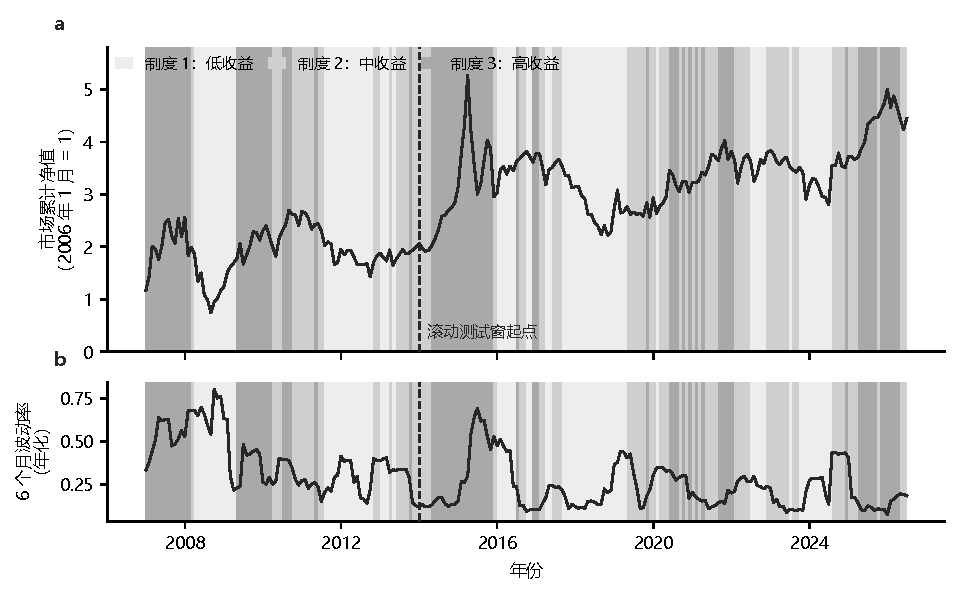
\includegraphics[width=\textwidth]{fig_regime.pdf}
\caption{样本期的市场环境与制度划分（2006--2026 年）}
\label{fig:regime}
\begin{minipage}{0.94\textwidth}\footnotesize
注：上图为市场累计净值（2006 年 1 月 = 1），底纹表示按 12 个月市场收益三分位
划分的制度状态；下图为 6 个月滚动波动率（年化）。竖虚线标出滚动测试窗起点。
状态划分与后文使用的制度变量一致，样本为沪深 A 股月度收益（247 个月）。
\end{minipage}
\end{figure}

点时股票池规则。每月形成日按四条规则筛选，条件只使用形成日及之前的信息：
当月至少有 5 个交易日（剔除长期停牌）、非 ST 类证券、上市满 6 个月、
成交额处于横截面 30\% 分位以上。四条规则分别剔除流动性中断、特殊处理、
新股与低流动性证券。

退市处理。证券列表包含已退市与已摘牌证券。有执行价但随后无行情的观测，
收益记为 $-1$，以控制幸存者偏差。本文区分两种情形：真实退市指有执行价但因数据中断
而没有退出价，收益记 $-1$；数据右边界指最后一个观测月及其前一月，
其退出价落在尚未观测到的下一个月，该整月从样本中剔除，以保证横截面在月份间可比。
样本中的真实退市观测为 8 个。公开行情接口对部分早期退市证券已不提供历史数据，
退市损失的覆盖因此偏低，结果相对乐观；由于本文的核心结论是门控优势不显著，
这一方向性偏差不改变主要判断（第 \ref{sec:robust} 节详述）。

执行采用严格点时规则：$t$ 月末收盘观测全部特征与市场状态，形成目标权重 $w_t$；
$t+1$ 月第一个交易日收盘按该日价格建仓；持有至 $t+2$ 月第一个交易日收盘换仓。
单期持有收益为后复权价之比。该规则比「月末收盘直接成交」保守，
不允许策略利用月末最后一个交易日的收盘价立即建仓，避免信号与成交价同时可观测的隐性前视。

换手按漂移后权重与目标权重之差的半 $L_1$ 范数计算，
交易成本为单边 $\kappa=10$ 个基点，从当期收益中扣除。
第 \ref{sec:marginal} 节与第 \ref{sec:robust} 节报告 $\kappa\in\{0,5,10,20,30,50\}$
基点的边际效应与敏感性。执行月首三个交易日触及涨停的证券标记为不可买入，
其权重按剩余可交易证券的比例再分配，使回测不依赖无法成交的价格；
涨跌停幅度按板块设定，科创板与创业板为 20\%，其余为 10\%。

本文的多智能体策略由五个专家智能体与一个门控智能体构成。
五个专家智能体为线性可解释信号（表 \ref{tab:expert-def}），门控智能体负责按状态分配权重。
打分方向由金融理论设定，不参与自由训练。该约束同时保证参数可识别：
若专家参数与门控参数自由联合训练，式 \eqref{eq:softmax-expert} 的 softmax 映射
具有平移不变性（$\theta$ 与 $\theta+c\bone$ 给出同一组合），
门控可通过缩放 $\tau_k$ 复制专家的任意强度变化，参数不可识别。

\begin{table}[htbp]
\centering
\caption{专家信号定义}
\label{tab:expert-def}
\begin{threeparttable}
\small
\begin{tabular}{lll}
\toprule
专家 & 打分 & 经济含义 \\
\midrule
动量 & $0.7\,\mathrm{mom}_{12-1}+0.3\,\mathrm{mom}_{12}$ & 中期价格趋势 \\
反转 & $-1.0\,\mathrm{mom}_{1}$ & 短期过度反应修正 \\
低波动 & $-1.0\,\mathrm{vol}_{60}$ & 低风险异象 \\
低换手 & $0.4\,\mathrm{mom}_{12-1}-0.6\,\mathrm{turnover}_{20}$ & 低流动性溢价 \\
低 beta & $0.3\,\mathrm{mom}_{12-1}-1.0\,\beta_{120}$ & 系统性风险规避 \\
\bottomrule
\end{tabular}
\begin{tablenotes}[flushleft]\footnotesize
\item 注：全部特征在每月横截面做 1\%--99\% 缩尾后标准化。
$\mathrm{mom}_{12-1}$ 为过去 12 个月剔除最近 1 个月的累计收益，
$\mathrm{mom}_{12}$ 为过去 12 个月累计收益，$\mathrm{mom}_{1}$ 为最近 1 个月收益；
$\mathrm{vol}_{60}$ 为 60 日收益标准差；$\mathrm{turnover}_{20}$ 为异常成交量
（20 日均量除以 250 日均量），因公开行情接口不提供换手率字段，以成交量口径替代；
$\beta_{120}$ 为 120 日滚动市场 beta。
\end{tablenotes}
\end{threeparttable}
\end{table}

打分经带温度参数 $\tau=0.6$ 的 softmax 映射为长仓满仓权重。
五个专家组合相对等权的平均半 $L_1$ 距离依次为：动量 0.431、反转 0.483、低波动 0.502、
低换手 0.336、低 beta 0.165，五个专家都产生了实质性不同于等权的持仓。
作为对照，梯度提升树策略的主动暴露仅为 0.005。

门控网络与训练目标。门控输入包含四组信息：市场制度变量（7 个）包括 3 个月与 12 个月市场收益、
6 个月波动率、6 个月趋势、1 年回撤、横截面离散度、上涨股票占比，
全部在训练窗内做扩展窗标准化；专家置信度为各专家截面打分的标准差；
专家风险为各专家组合的加权平均波动率；专家近期表现为指数加权历史收益
（衰减率 0.85），只使用当期之前的信息。门控为两层 tanh 网络（隐层 24 单元），
输出经 softmax 得到专家权重，组合自动满足长仓满仓约束。

训练目标为式 \eqref{eq:active-objective} 的主动收益型目标。信息比率项、CVaR 项
（5\% 尾部）、换手项与熵项的相对权重由验证窗在预先设定的 $3\times2$ 网格上选择，
测试窗不参与任何参数选择。门控网络的全部解析梯度经中心差分数值检验，
六种参数组合下的最大相对误差低于 $2\times10^{-6}$。该检验在实现过程中揭示了两类错误：
熵项与换手项缺失均值因子导致梯度按 $T$ 倍高估；标准差分母的数值稳定项经 $1/\sigma^3$
放大约 100 倍。两类错误均不导致程序报错，但会使训练结果无意义。

滚动样本外设计与推断。每个测试年份独立重估：训练窗为测试年前第 7 至第 2 年（5 年），
验证窗为测试年前 1 年，测试窗为测试当年。测试年份为 2014--2025 年，共 12 个年度窗口。
学习模型在每个窗口使用三个随机种子（7、19、42）重复，报告时先在年内对种子取平均，
再以年份为配对单位推断。相对基准的差异用循环区块自助法（块长 2 年，10\,000 次重抽样）
构造 95\% 区间，辅以 Wilcoxon 符号秩检验；对所有基准的多重比较采用 Holm 逐步校正；
模型整体排序差异用 Friedman 检验。随机种子用于度量优化不确定性，不作为额外的市场年份：
若把 3 个种子与 12 年当作 36 个独立观测，标准误将被低估约 $\sqrt{3}$ 倍。

互补性统计量由两个口径估计。第一个口径为月度横截面回归
\begin{equation}
r_{i,t+1}=a_t+\sum_{j=1}^J c_{j,t}\,\tilde x_{j,i,t}+\varepsilon_{i,t+1},
\label{eq:cs-regression}
\end{equation}
其中 $\tilde x_{j,i,t}$ 为第 $j$ 个特征在当月横截面标准化后的取值。
按制度归并回归系数 $c_{j,t}$ 得到 $\hat\Gamma^{\text{IC}}$。
第二个口径基于专家组合收益在制度内的均值与标准差，记为 $\hat\Gamma^{(1)}$
与 $\hat\Gamma^{(2)}$。

噪声底线的自校准用循环区块自助法：把制度标签在时间上做区块重抽样，
破坏制度与收益的对应关系，重新计算统计量，取分布的 95\% 分位数作为 $\Theta$。
该分布在无真实互补性时仍会因抽样噪声产生正值，其高分位数即「不可区分于噪声」的临界水平。
该设计不依赖式 \eqref{eq:theta-def} 中对 $\sigma_b$ 与 $\rho_k$ 的参数假设。
两个技术要点：$K$ 个专家的收益在横截面上高度相关，重抽样按整期联合抽取；
区块长度需覆盖制度内部的序列相关，本文取 12 个月，其敏感性见第 \ref{sec:robust} 节。
此外，按专家收益的平均两两相关估计有效独立专家数
$\hat K_{\text{eff}}=K/[1+(K-1)\bar\rho]$，并据此对自助分布的离散度做保守校正。

Oracle 门控与安慰剂检验。Oracle 门控按
$g^{\text{oracle}}_{k,s}\propto\exp(\eta\bar a_k^\top\hat\bmu_s)$ 构造，
其中 $\hat\bmu_s$ 为训练窗内制度 $s$ 的资产平均持有期收益。它使用制度内真实条件期望收益，
不可实现，仅用于度量一阶互补性的可利用上界。安慰剂检验保持门控输入与专家权重不变，
把资产收益矩阵在时间维度做循环区块置换后重新训练门控，重复 200 次；
同时计算制度间的变异系数 $\mathrm{CV}^{(1)}$（条件均值）与 $\mathrm{CV}^{(2)}$
（条件波动），并用区块置换构造零分布。

\section{实证结果：影响因素}
\label{sec:factors}

本节报告门控组合的基准表现，说明识别策略，并逐个检验四类影响因素：
训练目标、市场环境（含外生冲击）、收益来源渠道与制度持续性。

\begin{table}[htbp]
\centering
\caption{滚动样本外表现（2014--2025 年）}
\label{tab:main}
\begin{threeparttable}
\footnotesize
\begin{tabular}{lrrrr}
\toprule
\multicolumn{5}{l}{\textit{Panel A：收益与风险}} \\
模型 & CAGR & 波动率 & 夏普 & Sortino \\
\midrule
低波动专家 & 0.1285 & 0.1879 & 0.804 & 1.729 \\
风险平价 & 0.1216 & 0.2033 & 0.769 & 1.638 \\
门控组合（主动目标） & 0.1443 & 0.2376 & 0.673 & 2.779 \\
反转专家 & 0.1086 & 0.2691 & 0.579 & 2.055 \\
梯度提升树 & 0.0960 & 0.2369 & 0.566 & 2.148 \\
岭回归 & 0.0955 & 0.2367 & 0.563 & 2.130 \\
等权基准 & 0.0946 & 0.2368 & 0.558 & 2.141 \\
静态专家合成 & 0.1052 & 0.2349 & 0.547 & 1.045 \\
低换手专家 & 0.1018 & 0.2419 & 0.491 & 2.429 \\
动量专家 & 0.1144 & 0.2733 & 0.369 & 0.632 \\
低 beta 专家 & 0.0656 & 0.2410 & 0.351 & 1.528 \\
\bottomrule
\end{tabular}

\vspace{0.5em}
\begin{tabular}{lrrr}
\toprule
\multicolumn{4}{l}{\textit{Panel B：交易摩擦与主动暴露}} \\
模型 & 最大回撤 & 换手率 & 主动暴露 \\
\midrule
低波动专家 & $-0.120$ & 0.257 & 0.488 \\
风险平价 & $-0.133$ & 0.213 & 0.334 \\
门控组合（主动目标） & $-0.155$ & 0.372 & 0.309 \\
反转专家 & $-0.189$ & 0.618 & 0.490 \\
梯度提升树 & $-0.164$ & 0.131 & 0.005 \\
岭回归 & $-0.164$ & 0.131 & 0.005 \\
等权基准 & $-0.164$ & 0.131 & 0.000 \\
静态专家合成 & $-0.164$ & 0.289 & 0.242 \\
低换手专家 & $-0.171$ & 0.297 & 0.315 \\
动量专家 & $-0.197$ & 0.426 & 0.427 \\
低 beta 专家 & $-0.176$ & 0.185 & 0.164 \\
\bottomrule
\end{tabular}
\begin{tablenotes}[flushleft]\footnotesize
\item 注：样本为沪深 A 股点时面板，频率为月度，测试年份 2014--2025 年共 12 个年度窗口，
每个窗口独立重估（训练 5 年、验证 1 年）；学习模型在每个窗口使用三个随机种子并先取平均。
收益指标扣除单边 10 个基点的交易成本。主动暴露为组合权重相对等权的半 $L_1$ 距离均值，
取值范围为 0 至 1，等权组合取 0。2014 年前的年份用于训练与验证，不进入报告。
\end{tablenotes}
\end{threeparttable}
\end{table}

表 \ref{tab:main} 显示，门控组合的主动调整是实质性的：主动暴露为 0.309，
平均约 31\% 的组合权重偏离等权。梯度提升树与岭回归的主动暴露仅为 0.005。
在这两个模型中，直接预测收益再映射为权重的做法产生极端集中的权重，
在不可交易与成本约束下退化为近似等权。若研究者只报告夏普比率而不报告主动暴露，
读者无法区分自适应机制奏效与机制退化。

门控组合取得最高的年化收益（14.43\%）与最高的 Sortino 比率（2.779），
夏普比率 0.673 高于等权基准 0.558 与静态专家合成 0.547。其波动率（0.238）
略高于等权（0.237），收益改善并非来自降杠杆。五个专家信号表现分化明显：
低波动专家（0.804）与风险平价（0.769）优于门控组合，动量专家（0.369）与
低 beta 专家（0.351）明显落后。信号集合的高度异质性正是门控机制的设计场景。

\begin{table}[htbp]
\centering
\caption{相对等权基准的夏普差值检验（配对单位：测试年份，$n=12$）}
\label{tab:signif}
\begin{threeparttable}
\footnotesize
\begin{tabular}{lrrrrc}
\toprule
模型 & 差值 & 95\% 区间下限 & 95\% 区间上限 & 区间含零 & Holm 校正 $p$ \\
\midrule
低波动专家 & $+0.246$ & $+0.123$ & $+0.375$ & 否 & 0.041 \\
风险平价 & $+0.211$ & $+0.130$ & $+0.298$ & 否 & 0.017 \\
门控组合 & $+0.115$ & $-0.006$ & $+0.225$ & 是 & 0.386 \\
反转专家 & $+0.021$ & $-0.109$ & $+0.154$ & 是 & 1.000 \\
梯度提升树 & $+0.008$ & $+0.005$ & $+0.011$ & 否 & 0.005 \\
岭回归 & $+0.005$ & $+0.003$ & $+0.007$ & 否 & 0.009 \\
静态专家合成 & $-0.012$ & $-0.097$ & $+0.064$ & 是 & 1.000 \\
低换手专家 & $-0.067$ & $-0.224$ & $+0.062$ & 是 & 1.000 \\
动量专家 & $-0.190$ & $-0.442$ & $+0.021$ & 是 & 0.934 \\
低 beta 专家 & $-0.207$ & $-0.337$ & $-0.102$ & 否 & 0.009 \\
\bottomrule
\end{tabular}
\begin{tablenotes}[flushleft]\footnotesize
\item 注：区间由循环区块自助法（块长 2 年，10\,000 次重抽样）构造；
$p$ 值为 Wilcoxon 符号秩检验并作 Holm 多重比较校正。Friedman 检验统计量 39.11
（$p<0.001$），模型整体排序存在差异。
\end{tablenotes}
\end{threeparttable}
\end{table}

表 \ref{tab:signif} 报告的夏普差值为 $+0.115$，95\% 区间 $[-0.006,0.225]$，
Wilcoxon $p=0.077$，Holm 校正后 $p=0.386$；对应年化主动收益 3.77\%、
主动信息比率 0.80。门控组合的经济量级明显，统计显著性不足。
低波动专家与风险平价的优势在 5\% 水平上稳健显著（Holm $p=0.041$ 与 $0.017$）。

梯度提升树与岭回归的 Holm $p$ 值分别为 0.005 与 0.009，低于门控组合，
但其绝对量级仅为 $+0.008$ 与 $+0.005$，主动暴露接近零。这两个估计的显著性来自
极小的方差，对应的经济优势有限。仅依赖 $p$ 值判断会得出与量级相反的排序，
本文因此同时报告经济量级与主动暴露。

风险维度提供了另一组信息。门控组合相对等权的日频 5\% CVaR 改善为 $+0.0047$
（95\% 区间 $[-0.0087,0.0181]$），换手率提高 $+0.241$（Holm $p=0.005$）。
门控以显著更高的交易强度换取了幅度有限、与零不可区分的尾部风险改善。
这一取舍是第 \ref{sec:policy} 节讨论风险管理含义的基础。
\begin{figure}[htbp]
\centering
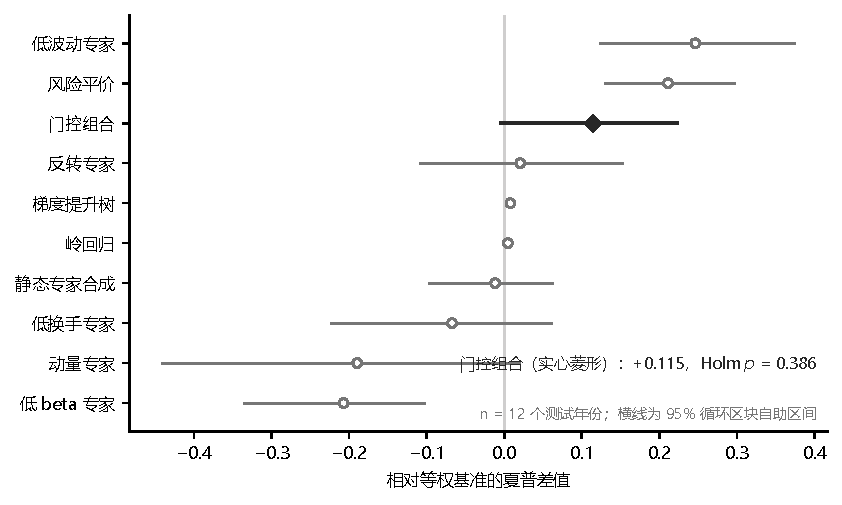
\includegraphics[width=0.82\textwidth]{fig_significance.pdf}
\caption{各模型相对等权基准的夏普差值}
\label{fig:significance}
\begin{minipage}{0.9\textwidth}\footnotesize
注：标记为夏普差值的点估计，横线为循环区块自助法（块长 2 年，10\,000 次重抽样）
构造的 95\% 区间，配对单位为测试年份（$n=12$）；实心菱形为门控组合。
区间跨越零的模型，其优势与零不可区分。
\end{minipage}
\end{figure}

识别策略。门控价值的因果解释面临两个威胁：门控收益可能来自样本内过拟合，
也可能来自与制度无关的风险暴露。本文用三层设计逐一排除。

第一层是随机化推断。按推论 \ref{cor:identification}，
破坏制度与收益的对应关系后门控收益应当归零。本文保持门控输入形式与专家权重不变，
对收益矩阵做循环区块置换并重新训练门控，重复 200 次，得到门控收益的零分布。
该层识别的是制度信息对收益的必要性。

第二层是上界检验。Oracle 门控使用制度内真实条件期望收益，
给出利用一阶互补性所能达到的上界。若门控收益来自收益择时的预测能力，
其表现不应超过该上界。该层识别的是收益来源渠道。

第三层是外生冲击分组。制度切换的时点若由市场内生决定，
「门控在制度切换后表现更好」存在反向因果的可能。
本文改用事件时间外生的冲击年份作为分组变量（政策与国际事件的发生时点不依赖模型），
比较冲击年与对照年的门控价值，并同时检查两组的波动率与切换次数，
以区分状态分化幅度与切换频率两个渠道。

三层设计对应三个识别对象：制度信息的必要性、收益来源渠道、价值的时点分布。
任何单层都不足以构成因果论证，合起来可以排除过拟合、渠道误判与内生时点三个主要解释。
识别仍依赖的前提是：专家信号的方向由理论事先设定、不参与自由训练；
门控只在训练窗内拟合，验证窗选超参，测试窗仅用于评估。

\begin{table}[htbp]
\centering
\caption{训练目标对门控行为的影响}
\label{tab:degeneracy}
\begin{threeparttable}
\footnotesize
\begin{tabular}{p{2.9cm}rrrp{2.4cm}}
\toprule
训练目标 & 主动暴露 & 平均换手率 & 相对等权的夏普差 & 结论 \\
\midrule
绝对收益（常见做法） & $\approx0.0003$ & 0.0029 & $-0.001$（含零，$p=1.000$） & 退化为静态等权 \\
主动收益（本文修正） & 0.309 & 0.372 & $+0.115$（含零，$p=0.077$） & 实质动态调整 \\
\bottomrule
\end{tabular}
\begin{tablenotes}[flushleft]\footnotesize
\item 注：绝对收益目标的行为来自以十只美国 ETF 为样本的设定；
主动收益目标的行为来自本文的 A 股主实验。主动暴露为组合权重相对等权的半 $L_1$ 距离。
\end{tablenotes}
\end{threeparttable}
\end{table}

表 \ref{tab:degeneracy} 对比两种训练目标下的门控行为，用于检验命题 \ref{prop:degeneracy}。
绝对收益目标下，主动暴露约为 $0.0003$，组合几乎恒等于等权；换手率 0.0029
与静态持有水平相当；夏普比率与等权基准无法区分。目标函数中与决策无关的基准收益项
主导梯度，是该行为的直接来源。改为主动收益目标后，主动暴露上升约三个数量级至 0.309，
门控具备识别互补性的条件。

这一对照的适用范围超出本文样本。在满仓长仓约束下，训练目标的选择决定自适应机制
能否偏离静态基准，其影响先于网络架构的设计。使用绝对收益目标的同类研究，
若不报告主动暴露，其零结果可能来自目标函数设计而非机制无效。报告自适应组合表现时
同时报告主动暴露，可以把这一来源区分开。

\begin{table}[htbp]
\centering
\caption{年度市场环境与门控组合的相对表现}
\label{tab:year-env}
\begin{threeparttable}
\footnotesize
\begin{tabular}{lrrrrrrr}
\toprule
年份 & 市场收益 & 市场波动率 & 制度切换次数 & 横截面离散度
& 门控夏普 & 等权夏普 & 夏普差值 \\
\midrule
2014 & 0.427 & 0.148 & 1 & 0.105 & 2.587 & 2.491 & $+0.096$ \\
2015 & 0.040 & 0.575 & 1 & 0.137 & 0.515 & 0.367 & $+0.148$ \\
2016 & 0.224 & 0.177 & 5 & 0.090 & 1.410 & 1.221 & $+0.189$ \\
2017 & $-0.135$ & 0.188 & 4 & 0.091 & $-0.497$ & $-0.682$ & $+0.185$ \\
2018 & $-0.271$ & 0.176 & 0 & 0.091 & $-1.445$ & $-1.691$ & $+0.246$ \\
2019 & 0.127 & 0.328 & 3 & 0.102 & 0.722 & 0.509 & $+0.214$ \\
2020 & 0.187 & 0.285 & 7 & 0.124 & 1.030 & 0.725 & $+0.305$ \\
2021 & 0.203 & 0.165 & 6 & 0.130 & 1.554 & 1.199 & $+0.355$ \\
2022 & 0.034 & 0.241 & 3 & 0.120 & 0.186 & 0.210 & $-0.024$ \\
2023 & $-0.233$ & 0.164 & 3 & 0.088 & $-1.790$ & $-1.523$ & $-0.267$ \\
2024 & 0.208 & 0.324 & 2 & 0.115 & 0.786 & 0.698 & $+0.088$ \\
2025 & 0.347 & 0.096 & 4 & 0.112 & 3.013 & 3.174 & $-0.162$ \\
\bottomrule
\end{tabular}
\begin{tablenotes}[flushleft]\footnotesize
\item 注：市场收益为上证与深证综合口径的年度累计收益，市场波动率为月度收益标准差年化，
制度切换次数为 12 个月市场收益三分位制度在年内发生变化的次数，
横截面离散度为个股月收益横截面标准差的时间均值。门控夏普为三个随机种子的年内均值。
\end{tablenotes}
\end{threeparttable}
\end{table}

表 \ref{tab:year-env} 与图 \ref{fig:determinants} 报告门控相对价值的年度分布。
门控的相对价值随市场分化程度上升。年度波动率最低的三分之一年份，
夏普差值平均为 $+0.006$；中间三分之一为 $+0.149$；最高的三分之一为 $+0.189$，
秩相关系数为 0.259。横截面离散度呈现同向特征：最低三分之一为 $+0.088$，
最高三分之一为 $+0.196$，秩相关为 0.231。市场方向不解释门控价值：
年度收益与差值的秩相关为 $-0.049$，年度最大回撤为 0.042。
门控价值来自市场状态的分化程度，而非市场涨跌。

\begin{figure}[htbp]
\centering
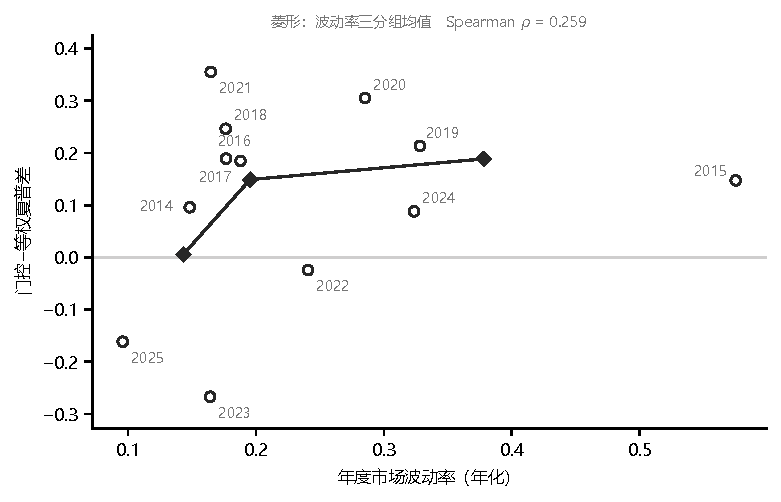
\includegraphics[width=0.78\textwidth]{fig_determinants.pdf}
\caption{年度市场波动率与门控组合的相对优势（2014--2025 年）}
\label{fig:determinants}
\begin{minipage}{0.86\textwidth}\footnotesize
注：散点为 12 个测试年份，纵轴为门控组合相对等权基准的夏普差值；
折线为按年度波动率三分组的组内均值。$N=12$。
\end{minipage}
\end{figure}

年度观测只有 12 个，单变量回归不足以支持因果推断，上述分组特征作为门控优势
在时间上分布不均衡的证据，其方向与「制度条件信息在高波动、高分化环境下更有价值」
的机制一致。

外生冲击下的门控价值。表 \ref{tab:year-env} 的分组变量由市场统计量构造，可能与门控表现同时受第三方因素影响。
本节改用事件时间外生的冲击年份作分组，冲击的发生时点由政策与国际事件决定，
不依赖模型与策略。

\begin{table}[htbp]
\centering
\caption{外生冲击年与对照年的门控价值}
\label{tab:shock}
\begin{threeparttable}
\small
\begin{tabular}{lrrrr}
\toprule
分组 & 夏普差值均值 & 市场波动率 & 制度切换次数 & 横截面离散度 \\
\midrule
冲击年（5 个） & $+0.173$ & 0.291 & 3.20 & 0.112 \\
对照年（7 个） & $+0.073$ & 0.202 & 3.29 & 0.106 \\
\midrule
\multicolumn{5}{l}{差值（年份聚类自助，2\,000 次）：
$+0.100$，95\% 区间 $[-0.081,0.276]$，$p=0.298$} \\
\bottomrule
\end{tabular}
\begin{tablenotes}[flushleft]\footnotesize
\item 注：冲击年为 2015、2016、2018、2020、2022 年，依次对应股市异常波动、
熔断机制实施、中美贸易摩擦、新冠疫情、俄乌冲突与疫情封控，
事件时点由外部事件日历确定；其余 7 年为对照年。
市场波动率为月度收益标准差年化，制度切换次数为 12 个月市场收益三分位制度
在年内发生变化的次数，横截面离散度为个股月收益横截面标准差的时间均值。
夏普差值为门控组合相对等权基准的差值。
\end{tablenotes}
\end{threeparttable}
\end{table}

冲击年的门控相对优势为 $+0.173$，对照年为 $+0.073$，差值为 $+0.100$
（95\% 区间 $[-0.081,0.276]$）。点估计方向与「外生冲击提高状态分化程度、
从而提高门控价值」的推断一致，区间的宽度说明 12 个年度观测下的识别能力有限。
两组的分组特征给出机制信息：冲击年的市场波动率为 0.291，明显高于对照年的 0.202；
制度切换次数几乎相同（3.20 对 3.29）；横截面离散度略高（0.112 对 0.106）。
门控价值与状态分化的幅度同向，与制度切换的频率关系不大，
这与前文的结果一致。该模式同时排除一类解释：
门控收益并非来自频繁调仓本身。

门控的可实施性还取决于状态能否实时识别。若状态切换可以被事前预判，
策略可以通过择时调仓规避高成本时段；若不能，门控的价值只能来自识别当前状态并利用其持续性。
本文用 logit 与 probit 模型检验这一问题，被解释变量为下月状态，
解释变量为滞后一期的公开信息，结果见表 \ref{tab:logit}。

三个结果值得注意。制度切换基本不可预测：伪 $R^2$ 为 0.04，
样本内命中率 0.53 低于「始终预测不切换」的 0.76，切换时点没有可用的公开前兆。
状态本身具有很强的判别力：风险结构制度的伪 $R^2$ 为 0.45、样本外命中率 0.87，
收益水平制度为 0.41、0.75。判别力的来源符合渠道分解：
风险结构制度的主要判别变量是滞后波动率（平均边际效应 $+0.194$，$p<0.001$），
即波动聚集；收益水平制度的主要判别变量是滞后回撤（$-0.314$，$p<0.001$）
与横截面离散度（$-0.138$，$p<0.001$），其余变量的边际效应在 10\% 水平上不显著。

这组结果与持续性乘数一致：状态的价值来自其持续性，而非对切换时点的预知。
门控因此是可实施的——策略不需要预测何时切换，只需在每月识别当前状态；
但它也无法通过择时规避切换带来的换手成本，这与第 \ref{sec:marginal} 节的
成本敏感性结果互相呼应。

\begin{table}[htbp]
\centering
\caption{状态可预测性检验（被解释变量：下月状态）}
\label{tab:logit}
\begin{threeparttable}
\footnotesize
\begin{tabular}{lrrrr}
\toprule
被解释变量 & 模型 & 伪 $R^2$ & 样本内命中率 & 样本外命中率 \\
\midrule
风险结构制度（高波动） & logit & 0.449 & 0.834 & 0.874 \\
风险结构制度（高波动） & probit & 0.436 & 0.834 & 0.869 \\
收益水平制度（熊市） & logit & 0.406 & 0.809 & 0.754 \\
收益水平制度（熊市） & probit & 0.413 & 0.809 & 0.760 \\
制度切换（收益水平划分） & logit & 0.041 & 0.528 & 0.726 \\
制度切换（收益水平划分） & probit & 0.042 & 0.532 & 0.726 \\
\midrule
\multicolumn{5}{l}{基准率：风险结构制度 0.32、收益水平制度 0.34、制度切换 0.24} \\
\bottomrule
\end{tabular}
\begin{tablenotes}[flushleft]\footnotesize
\item 注：样本为 2006--2026 年 235 个月度观测；解释变量为滞后一期的公开信息
（上月市场收益、近 3 个月收益、近 6 个月波动、近 1 年回撤、横截面离散度、
上涨股票占比），均做标准化处理；标准误为 Newey--West（6 阶）。
样本外命中率为扩展窗逐步预测的结果，训练起点为第 60 个月。
基准率指被解释变量取 1 的无条件频率。
\end{tablenotes}
\end{threeparttable}
\end{table}

\begin{table}[htbp]
\centering
\caption{信号—状态互补性与估计噪声底线}
\label{tab:gamma}
\begin{threeparttable}
\small
\begin{tabular}{llrrrr}
\toprule
估计口径 & 渠道 & 统计量 & 噪声底线 $\Theta$ & $p$ 值 & 是否越过 5\% \\
\midrule
截面回归 IC & 一阶 & $4.0\times10^{-6}$ & $1.4\times10^{-5}$ & 0.708 & 否 \\
专家组合收益 & 一阶 & $3.93\times10^{-4}$ & $4.17\times10^{-4}$ & 0.060 & 否（临界） \\
专家组合收益 & 二阶 & $6.34\times10^{-4}$ & $6.87\times10^{-4}$ & 0.065 & 否（临界） \\
\midrule
\multicolumn{2}{l}{美国 ETF 10 只（$N=10$）} & \multicolumn{3}{r}{不可识别} & —— \\
\bottomrule
\end{tabular}
\begin{tablenotes}[flushleft]\footnotesize
\item 注：$\Theta$ 由循环区块自助法在「无真实互补性」原假设下校准
（块长 6--12 个月，500 次重抽样），取统计量分布的 95\% 分位数；
$p$ 值为自助分布中不小于观测值的比例。窄横截面样本因每月证券数不足 20 只
而无法估计月度横截面回归。
\end{tablenotes}
\end{threeparttable}
\end{table}

表 \ref{tab:gamma} 的三种口径给出一致结果：互补性统计量均未越过 5\% 水平的噪声底线，
两种专家组合收益口径接近临界（一阶 $p=0.060$，二阶 $p=0.065$）。
在 12 个测试年份、247 个月度观测下，条件信息系数的制度间差异刚好处在
可与抽样噪声区分的边缘。该结果与表 \ref{tab:signif} 中 $+0.115$ 的夏普差值互相印证，
两套独立检验给出同一个位置判断：门控运行在阈值附近。

\begin{table}[htbp]
\centering
\caption{渠道识别：Oracle 上界、安慰剂与变异系数检验}
\label{tab:oracle}
\begin{threeparttable}
\small
\begin{tabular}{lrrr}
\toprule
检验 & 夏普 & 年化收益 & 换手率 \\
\midrule
等权基准 & 0.558 & 9.5\% & 0.131 \\
静态专家合成 & 0.546 & 10.5\% & 0.289 \\
Oracle 门控（用真实条件期望收益） & 0.562 & 10.7\% & 0.291 \\
\midrule
\multicolumn{4}{l}{\textit{安慰剂检验（区块置换收益—制度关联，200 次）}} \\
门控主动收益 & \multicolumn{3}{r}{$+0.004\%$，95\% 区间 $[-0.413\%,+0.357\%]$} \\
\midrule
\multicolumn{4}{l}{\textit{渠道识别检验（区块置换，1\,000 次，块长 12 月）}} \\
一阶变异系数 $\mathrm{CV}^{(1)}$ & \multicolumn{3}{r}{观测 2.722 vs 零分布均值 0.450，$p=0.001$} \\
二阶变异系数 $\mathrm{CV}^{(2)}$ & \multicolumn{3}{r}{观测 0.104 vs 零分布均值 0.022，$p=0.003$} \\
\bottomrule
\end{tabular}
\begin{tablenotes}[flushleft]\footnotesize
\item 注：Oracle 门控按训练窗内各制度的资产平均持有期收益为专家加权，
使用真实条件期望收益，不可实现，仅用于构造一阶互补性的可利用上界。
变异系数定义为制度间方差除以均值平方。
\end{tablenotes}
\end{threeparttable}
\end{table}

表 \ref{tab:oracle} 的三类检验依次确定收益的制度依赖、来源渠道与状态依赖强度。
安慰剂检验把门控主动收益由 3.77\% 压至 0.004\%（95\% 区间 $[-0.413\%,+0.357\%]$），
按推论 \ref{cor:identification}，门控收益依赖制度信息，不是样本内过拟合或随机噪声。
Oracle 门控的夏普比率为 0.562，与等权基准（0.558）和静态专家合成（0.546）几乎无差异：
即使允许门控使用各制度内真实的条件期望收益，表现也没有改善，
数据中可利用的一阶互补性有限。渠道识别检验显示制度间变异系数远超置换零分布，
一阶 $\mathrm{CV}^{(1)}$ 为 2.722（零分布均值 0.450，$p=0.001$），
二阶 $\mathrm{CV}^{(2)}$ 为 0.104（零分布均值 0.022，$p=0.003$），
两条渠道都存在显著的状态依赖。

三类检验合起来指向同一结论：状态依赖存在，可利用的一阶互补性有限，
门控收益主要来自二阶渠道，即通过识别制度相关的风险结构
（专家信号的波动率与相关性差异）重新配置风险，而非预测哪个专家在哪个制度下收益更高。
该结论有一个直接推论：若门控价值主要来自风险配置，更简单的风险结构策略应当同样有效。
表 \ref{tab:main} 与此一致：低波动专家（0.804）与风险平价（0.769）都是二阶渠道的
纯化形式，表现优于包含完整门控机制的组合（0.673）。

\begin{figure}[htbp]
\centering
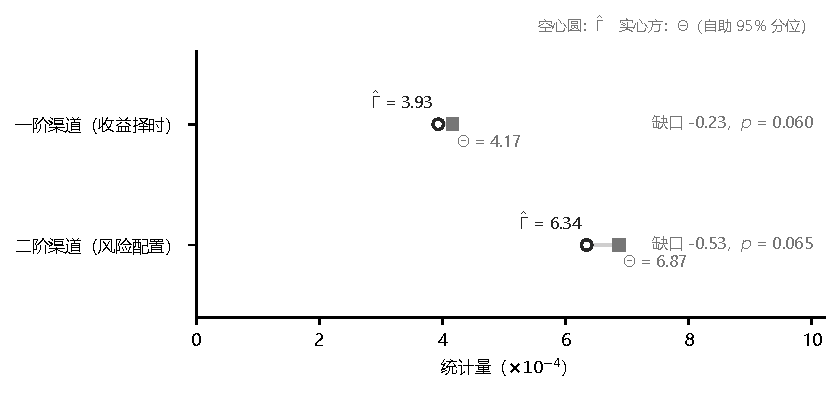
\includegraphics[width=0.62\textwidth]{fig_threshold.pdf}
\caption{互补性统计量与噪声底线的对照}
\label{fig:threshold}
\begin{minipage}{0.86\textwidth}\footnotesize
注：白色阴影柱为互补性统计量 $\hat\Gamma$，灰色柱为循环区块自助法校准的
噪声底线 $\Theta$（95\% 分位）。两条渠道的 $\hat\Gamma$ 均略低于 $\Theta$。
\end{minipage}
\end{figure}

\begin{table}[htbp]
\centering
\caption{制度转移矩阵与持续性乘数（三制度，按 12 个月市场收益分位划分）}
\label{tab:persistence}
\begin{threeparttable}
\small
\begin{tabular}{lrrrrr}
\toprule
& \multicolumn{3}{c}{转移概率} & 持续概率 & 半衰期（月） \\
\cmidrule(lr){2-4}
制度 & 下一期=1 & 下一期=2 & 下一期=3 & & \\
\midrule
1（熊市） & 0.829 & 0.171 & 0.000 & 0.829 & 3.70 \\
2（震荡） & 0.148 & 0.704 & 0.148 & 0.704 & 1.97 \\
3（牛市） & 0.024 & 0.133 & 0.843 & 0.843 & 4.07 \\
\midrule
\multicolumn{5}{l}{平稳分布} & (0.340, 0.339, 0.321) \\
\multicolumn{5}{l}{持续性乘数 $\mathcal{M}_s$（$\beta=0.98$）} & (19.81, 18.40, 19.16) \\
\multicolumn{5}{l}{$\Corr(\mathcal{M}_s,\ \Gamma^{(1)}_s)$} & 0.985 \\
\multicolumn{5}{l}{持续性加权 / 未加权 $\Gamma^{(1)}$} & $19.5\times$ \\
\bottomrule
\end{tabular}
\begin{tablenotes}[flushleft]\footnotesize
\item 注：半衰期 $h_s=\ln0.5/\ln p_{ss}$；
持续性乘数 $\mathcal{M}_s=[(I-\beta P)^{-1}]_{ss}$，度量掌握当前制度对未来
收益分布的信息价值。
\end{tablenotes}
\end{threeparttable}
\end{table}

中国 A 股的制度状态高度持续：表 \ref{tab:persistence} 中转移矩阵的对角线概率为
0.829、0.704、0.843，平均半衰期 3.25 个月。「当前制度」包含关于未来 1--4 个月
收益分布的实质信息，而非瞬时噪声。持续性乘数与制度条件互补性的相关系数为 0.985，
考虑持续性后加权互补性为未加权的 19.5 倍，与定理 \ref{thm:persistence} 的方向一致。
持续性放大的是门控价值的量级，不改变阈值判定，因为噪声底线同样受制度内样本量约束。
$S=3$ 时上述相关系数只有 3 个观测点，此处作为方向性证据，不作精确估计。

识别设计给出三点支持：安慰剂检验排除样本内过拟合，Oracle 上界排除收益择时主导，
外生冲击分组把价值的时点分布与状态分化幅度而非切换频率联系起来。
在此基础上，四类影响因素按作用次序排列：训练目标决定机制能否偏离静态基准，
是必要条件；市场分化程度决定相对价值的年度分布；收益来源渠道决定门控的可实现形式
是风险结构配置；制度持续性放大价值量级。前三类因素都指向同一判断：
门控的价值来自信号的制度差异，而非信号数量或模型复杂度。

\section{实证结果：边际效应}
\label{sec:marginal}

按定理 \ref{thm:threshold}，门控的相对优势是互补性、估计噪声与交易成本的函数。
本节对四个可操作的设计维度——交易成本、制度状态数、训练窗长度与横截面宽度——
估计边际效应。估计沿用主实验的滚动协议，在年份固定效应下计算斜率，
并以测试年份为聚类单位做 2\,000 次自助重抽样。

\begin{table}[htbp]
\centering
\caption{交易成本对门控相对优势的边际效应}
\label{tab:cost}
\begin{threeparttable}
\footnotesize
\begin{tabular}{lrrrr}
\toprule
单边成本 $\kappa$（基点） & 门控夏普 & 等权夏普 & 夏普差值 & 门控换手率 \\
\midrule
0 & 0.701 & 0.566 & $+0.135$ & 0.372 \\
5 & 0.690 & 0.562 & $+0.128$ & 0.372 \\
10 & 0.678 & 0.558 & $+0.120$ & 0.372 \\
20 & 0.656 & 0.550 & $+0.105$ & 0.372 \\
30 & 0.633 & 0.542 & $+0.091$ & 0.372 \\
50 & 0.588 & 0.526 & $+0.062$ & 0.372 \\
\midrule
\multicolumn{5}{l}{斜率（年份固定效应，年份聚类自助）：
$-0.001\,47$/基点，95\% 区间 $[-0.001\,72,-0.001\,21]$，$p<0.001$} \\
\multicolumn{5}{l}{每 10 个基点的边际效应：$-0.0147$；盈亏平衡成本（线性外推）：
约 92 个基点} \\
\bottomrule
\end{tabular}
\begin{tablenotes}[flushleft]\footnotesize
\item 注：数值为 12 个测试年份、3 个随机种子的均值（$N=216$）。
门控换手率（0.372）约为等权（0.131）的 2.8 倍，成本上升对门控的边际影响更大。
本表为与主实验同一协议的独立重跑，10 个基点处的基线差值为 $+0.120$，
与主实验的 $+0.115$ 相差 0.005，差异来自随机种子下训练过程的数值波动。
\end{tablenotes}
\end{threeparttable}
\end{table}

交易成本由 0 上升至 50 个基点，门控相对等权的夏普差值由 $+0.135$ 单调下降至
$+0.062$，降幅 54\%；斜率估计为每基点 $-0.001\,47$（$p<0.001$）。
每 10 个基点的成本上升使相对优势下降约 0.015。成本以
$2\lambda\kappa\mathcal{C}(\hat g)$ 的形式进入阈值，换手越高门槛越高，
实证方向与比较静态 H3 一致。线性外推显示相对优势在单边成本约 92 个基点时消失。
A 股主动权益基金的显性费率与隐性冲击成本之和通常低于这一水平，
高频调仓的小市值策略则可能接近该临界值。

零成本假设提供了另一条信息。即使 $\kappa=0$，门控相对等权的夏普差值也仅为 $+0.135$。
门控的表现限制不在交易成本：若限制来自成本项，降低换手即可改善；
而本文的阈值检验（$p=0.060$ 与 $0.065$）显示限制来自 $\hat\Gamma<\Theta$，
调整换手无法改变这一判断。

\begin{table}[htbp]
\centering
\caption{制度状态数的边际效应}
\label{tab:states}
\begin{threeparttable}
\footnotesize
\begin{tabular}{lrrrr}
\toprule
制度状态数 $S$ & 门控夏普 & 夏普差值 & 分段边际效应 & 理论净价值 $\Delta(S)$ \\
\midrule
2 & 0.602 & $+0.044$ & —— & $-9.23\times10^{-4}$ \\
3 & 0.682 & $+0.123$ & $S{:}\,2\to3$：$+0.079$ & $-1.02\times10^{-3}$ \\
4 & 0.668 & $+0.110$ & $S{:}\,3\to4$：$-0.014$ & $-1.11\times10^{-3}$ \\
\midrule
\multicolumn{5}{l}{线性斜率（年份固定效应）：$+0.032\,8$/状态，95\% 区间
$[0.000\,4,0.066\,1]$，$p=0.047$} \\
\bottomrule
\end{tabular}
\begin{tablenotes}[flushleft]\footnotesize
\item 注：状态按 12 个月市场收益的分位数划分，并以 one-hot 形式并入门控输入。
夏普为 12 个测试年份、2 个随机种子的平均（$N=72$）。
理论净价值按式 \eqref{eq:delta-S} 计算（$\lambda=5$，门控参数 200 个）；
其绝对水平受容量项量级影响，此处关注其随 $S$ 的变化方向。
线性斜率包含 $S=2$ 到 $S=3$ 的跃升，掩盖了转折点，分段边际效应更能反映内点最优。
\end{tablenotes}
\end{threeparttable}
\end{table}

门控表现在 $S=3$ 处达到最高（0.682），$S=2$ 时为 0.602，$S=4$ 时回落至 0.668，
呈内点最优。分段边际效应为 $2\to3$ 提升 0.079、$3\to4$ 下降 0.014，
边际收益在 $S=3$ 处转负。制度数增加提高可用互补性 $\Gamma(S)$，
同时提高估计误差成本 $\Theta(S)$ 与容量成本；当后者的边际成本超过前者的边际收益时，
净价值开始下降（定理 \ref{thm:optimal-S}）。

理论净价值与实证最优点存在定量差异。按式 \eqref{eq:delta-S} 使用名义门控参数量
（200 个）计算，净价值在所有 $S$ 下均为负，最优点落在 $S=2$，
容量项 $\sigma^2d_{\text{gate}}/T$ 以 $200/247$ 的量级主导了净价值。
该差异印证定理 \ref{thm:optimal-S} 的核心含义：在 $T=247$ 的样本量下，
200 个自由参数的门控处于容量约束的紧边界上。实证中最优的 $S=3$ 由验证窗在
$3\times2$ 网格中选出，其有效自由度远低于名义值。内点最优的方向得到支持，
精确定位需要更大样本或更小容量的门控架构。

\begin{table}[htbp]
\centering
\caption{训练窗长度的边际效应}
\label{tab:trainlen}
\begin{threeparttable}
\small
\begin{tabular}{lrrr}
\toprule
训练窗长度 & 窗口数 & 门控夏普 & 相对等权夏普差值 \\
\midrule
3 年 & 36 & 0.727 & $+0.213$ \\
5 年 & 36 & 0.678 & $+0.120$ \\
8 年 & 33 & 0.703 & $+0.163$ \\
\midrule
\multicolumn{4}{l}{线性斜率（年份固定效应）：$-0.006\,3$/年，
95\% 区间 $[-0.030\,8,0.018\,3]$，$p=0.617$} \\
\bottomrule
\end{tabular}
\begin{tablenotes}[flushleft]\footnotesize
\item 注：训练窗缩短减少门控的可用样本（提高 $\Theta$），
同时使训练数据更接近当前市场结构（降低结构变化带来的设定误差）。
样本窗口数因可用历史长度而异（$N=105$）。
\end{tablenotes}
\end{threeparttable}
\end{table}

训练窗长度。表 \ref{tab:trainlen} 不支持比较静态 H4 的简单形式。3 年训练窗的相对优势最高
（$+0.213$），8 年次之（$+0.163$），5 年最低（$+0.120$），呈非单调模式，
线性斜率的 95\% 区间跨越零。估计误差机制（$\Theta\propto1/T$）与结构变化机制
在此方向相反：更长的训练窗降低抽样误差，同时引入更多来自不同市场结构的陈旧信息，
提高设定误差。A 股在 2014--2026 年间经历注册制改革、涨跌停制度调整与投资者结构变化，
信号有效性随时间漂移，结构变化的力量在本样本中占优，最优训练窗长度约为 3 年。

该结果指向一个更一般的判断：定理 \ref{thm:threshold} 中的 $T$ 应理解为
来自同一数据生成过程的有效样本量，而非日历长度。
在结构变化明显的市场上，延长训练窗不必然降低 $\Theta$。
以「训练样本更长」为由扩大模型容量，在市场结构快速变化的环境下未必成立。

横截面宽度。横截面宽度与上述三个维度不同：它不可由研究者调节，却决定机制能否被识别。
两条渠道的噪声底线按不同速率收敛，$\Theta^{(1)}\asymp c_1(S-1)/T$，
$\Theta^{(2)}\asymp c_2(S-1)/(NT)$；互补性统计量的上界以 $1/N$ 收缩。
在宽横截面上，二阶渠道的噪声底线以 $1/N$ 的速率下降，识别能力显著改善；
扩大横截面对一阶渠道不带来识别增益。

本文的两个样本给出直接对照。A 股样本的平均横截面宽度约为 438 只，
互补性统计量处于阈值边缘（$p=0.060$ 与 $0.065$）；十只美国 ETF 的样本上，
月度横截面回归因每月证券数不足 20 只而无法估计，互补性检验不可识别。
后者的原因不是实现质量，而是 $\hat\Gamma$ 的上界因 $N=10$ 而低于噪声底线。
以少数 ETF 为样本、却报告多智能体门控优势的研究，在本文框架下面临这一识别问题。

\begin{figure}[htbp]
\centering
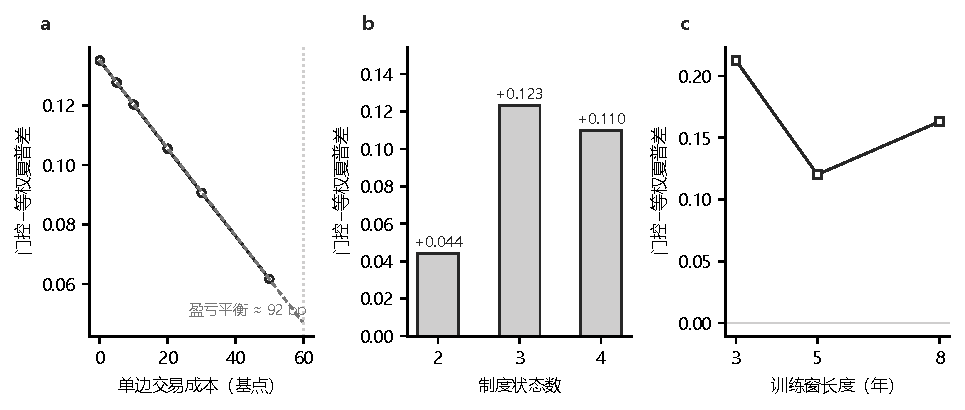
\includegraphics[width=\textwidth]{fig_marginal.pdf}
\caption{三个设计维度的边际效应}
\label{fig:marginal}
\begin{minipage}{0.94\textwidth}\footnotesize
注：(a) 交易成本：散点为各成本水平的夏普差值均值，虚线为年份固定效应下的线性拟合，
点线标出线性外推的盈亏平衡成本（约 92 个基点）；
(b) 制度状态数：由 2 增至 3 提升 0.079，由 3 增至 4 下降 0.014；
(c) 训练窗长度：3 年、5 年、8 年分别为 $+0.213$、$+0.120$、$+0.163$，非单调。
\end{minipage}
\end{figure}

\begin{table}[htbp]
\centering
\caption{边际效应估计汇总}
\label{tab:marginal-sum}
\begin{threeparttable}
\footnotesize
\begin{tabular}{lp{3.6cm}rrp{3.2cm}}
\toprule
维度 & 边际效应 & 95\% 区间 & $p$ 值 & 对应的理论含义 \\
\midrule
交易成本 & $-0.001\,47$/基点 & $[-0.001\,72,-0.001\,21]$ & $<0.001$ & H3：成本线性进入阈值 \\
\quad（换算） & $-0.0147$/10 基点 & —— & —— & 盈亏平衡约 92 基点 \\
制度状态数 & $+0.032\,8$/状态 & $[0.000\,4,0.066\,1]$ & 0.047 & H1：净价值单峰 \\
\quad（分段） & $2\to3$：$+0.079$；$3\to4$：$-0.014$ & —— & —— & 内点最优在 $S=3$ \\
训练窗长度 & $-0.006\,3$/年 & $[-0.030\,8,0.018\,3]$ & 0.617 & H4：不支持简单形式 \\
横截面宽度 & 不可调节 & —— & —— & 一阶 $\Theta\propto1/T$，二阶 $\Theta\propto1/(NT)$ \\
持续性乘数 & 放大 19.5 倍 & —— & —— & H5：$\mathcal{M}=(I-\beta P)^{-1}$ \\
\bottomrule
\end{tabular}
\begin{tablenotes}[flushleft]\footnotesize
\item 注：斜率均在年份固定效应下估计，以测试年份为聚类单位做 2\,000 次自助重抽样；
$p$ 值为对零的双侧自助检验。交易成本面板 $N=216$，制度数面板 $N=72$，
训练窗面板 $N=105$，均为测试年份与随机种子的组合。
\end{tablenotes}
\end{threeparttable}
\end{table}

四个维度的估计给出一个统一判断：门控的净价值对交易成本高度敏感，
对制度数呈内点最优，对训练窗长度不敏感。提高模型复杂度的边际回报很小甚至为负，
控制换手与成本、把制度数控制在样本量容许的范围内，才是提高净价值的关键。

\section{稳健性检验}
\label{sec:robust}

本节按时间稳定性、制度设定、推断方法与样本宽度四类威胁检验前述结论，
并对照既有零结果。

\begin{table}[htbp]
\centering
\caption{子样本稳定性}
\label{tab:subsample}
\begin{threeparttable}
\small
\begin{tabular}{llrrr}
\toprule
时段 & 年份 & 门控夏普 & 等权夏普 & 夏普差值 \\
\midrule
前半段 & 2014--2019 & 0.549 & 0.369 & $+0.180$ \\
后半段 & 2020--2025 & 0.797 & 0.747 & $+0.049$ \\
\bottomrule
\end{tabular}
\begin{tablenotes}[flushleft]\footnotesize
\item 注：数值由主实验的年度窗口直接汇总（与表 \ref{tab:main} 同源）。段内先对随机种子取平均，再对年份取平均。
\end{tablenotes}
\end{threeparttable}
\end{table}

表 \ref{tab:subsample} 显示门控优势的时间衰减：相对等权的夏普差值在前半段
（2014--2019）为 $+0.180$，在后半段（2020--2025）降至 $+0.049$。
两段内门控的绝对表现都上升（0.549 $\to$ 0.797），等权基准上升更多
（0.369 $\to$ 0.747），相对优势因此收窄。两个机制可以解释这一模式：
2014--2019 年 A 股经历若干次幅度较大的制度切换（2015 年杠杆牛市与随后的调整、
2016 年熔断），状态识别的价值较高；2020 年后风格切换更频繁但幅度更温和，
且股票池由 428 只扩大至 523 只，等权基准的分散化程度提高。
无论何种解释，基于全样本平均的门控优势结论都需要补充子样本稳定性。

\begin{table}[htbp]
\centering
\caption{制度定义与制度数的稳健性}
\label{tab:statedef}
\begin{threeparttable}
\small
\begin{tabular}{llrr}
\toprule
制度变量 & 制度数 & 平均夏普 & 相对等权夏普差值 \\
\midrule
12 个月市场收益 & 2 & 0.631 & $+0.073$ \\
12 个月市场收益 & 3 & 0.722 & $+0.164$ \\
6 个月市场波动 & 2 & 0.668 & $+0.110$ \\
6 个月市场波动 & 3 & 0.618 & $+0.060$ \\
1 年市场回撤 & 2 & 0.702 & $+0.144$ \\
1 年市场回撤 & 3 & 0.561 & $+0.003$ \\
横截面离散度 & 2 & 0.705 & $+0.147$ \\
横截面离散度 & 3 & 0.619 & $+0.060$ \\
\bottomrule
\end{tabular}
\begin{tablenotes}[flushleft]\footnotesize
\item 注：制度以 one-hot 形式并入门控输入，其余设定不变。
数值为 12 个测试年份的平均（单一种子）。差值为相对同期等权基准的夏普差。
\end{tablenotes}
\end{threeparttable}
\end{table}

表 \ref{tab:statedef} 显示结果对制度定义敏感。夏普表现区间为 0.561（1 年回撤，$S=3$）
至 0.722（12 个月收益，$S=3$），跨度约 0.16，与门控相对等权的整体优势（$+0.12$）
同量级，制度变量的选择本身贡献了与机制同量级的不确定性。
「12 个月市场收益 + 3 状态」在 $S=2$ 与 $S=3$ 下表现均较好，
其余三种定义下 $S=2$ 优于 $S=3$，说明在这些定义下增加制度数带来的估计误差成本
超过互补性收益。相对优势在八种设定下全部为正（$+0.003$ 至 $+0.164$），
收益方向不依赖特定定义，量级则高度依赖定义。

\begin{table}[htbp]
\centering
\caption{自助区块长度对阈值检验的影响}
\label{tab:block}
\begin{threeparttable}
\small
\begin{tabular}{lrrr}
\toprule
区块长度（月） & 一阶 $p$ 值 & 二阶 $p$ 值 & 5\% 水平是否显著 \\
\midrule
3 & 0.055 & 0.018 & 仅二阶 \\
6 & 0.048 & 0.030 & 一阶与二阶 \\
12 & 0.060 & 0.065 & 均不显著 \\
24 & 0.060 & 0.095 & 均不显著 \\
\bottomrule
\end{tabular}
\begin{tablenotes}[flushleft]\footnotesize
\item 注：$p$ 值为自助分布中不小于观测统计量的比例。区块越长，
保留的序列相关越多，噪声底线越高，检验越保守。
\end{tablenotes}
\end{threeparttable}
\end{table}

阈值检验的结论依赖区块长度（表 \ref{tab:block}）。区块长度为 3--6 个月时，
至少一条渠道在 5\% 水平上显著；12--24 个月时两条渠道均不显著。
区块长度的选择依据是制度内部序列相关的实际长度。本文估计的制度平均半衰期为
3.25 个月（表 \ref{tab:persistence}），而专家收益的自相关还来自动量类信号本身的持续性，
动量信号在 6--12 个月尺度上仍存在自相关，区块长度至少应覆盖 12 个月。
本文主结果采用 12 个月的保守设定。该敏感性说明门控优势的统计显著性处于
视推断方法而定的边缘地带，与门控运行在阈值附近的判断一致。
多智能体组合的业绩评估应当预先注册推断方法，避免区块长度、
配对单位等研究者自由度改变结论。
\begin{figure}[htbp]
\centering
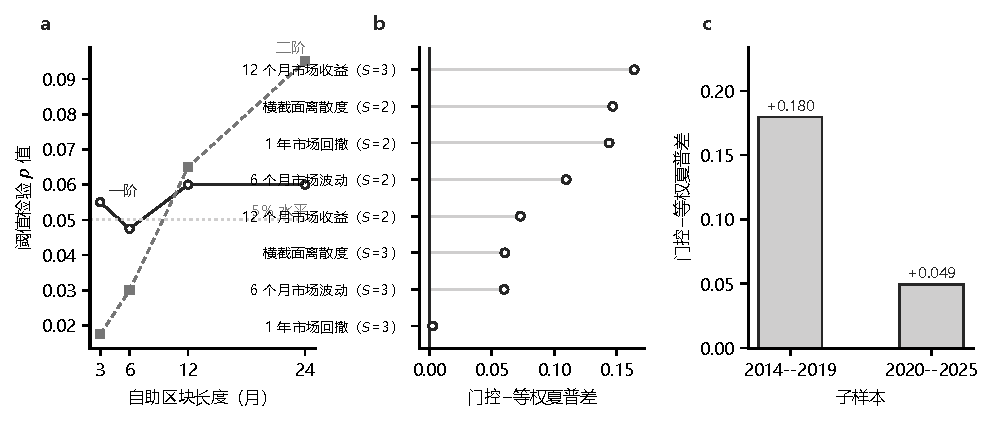
\includegraphics[width=\textwidth]{fig_robustness.pdf}
\caption{稳健性检验汇总}
\label{fig:robustness}
\begin{minipage}{0.94\textwidth}\footnotesize
注：(a) 阈值检验的 $p$ 值随自助区块长度变化，点线为 5\% 水平，一阶与二阶渠道
分别用实线圆点与虚线方点表示；(b) 四种制度变量与两种制度数下相对同期等权基准的
夏普差值；(c) 子样本的夏普差值均值，由主实验年度窗口汇总。
\end{minipage}
\end{figure}

十只美国 ETF 样本上的不可识别结果还有一层对照意义：该样本正是既有研究报告
「门控与等权不可区分」结论的样本。本文在该样本上重复得到相同结论，
并给出三重解释：绝对收益目标使门控退化（主动暴露 $0.0003$）；
横截面过窄使互补性统计量的上界低于噪声底线；样本期内制度持续性与互补性
都不足以支撑门控优势。既有实验的零结果在本文框架下对应三个具体预测的同时成立。
以少数资产为标的的多智能体研究与股票横截面研究之间，结论不宜互相外推。

本文结论受四项数据约束。样本覆盖方面，868 只证券来自公开行情接口在采集期内
仍可返回历史数据的证券集合，覆盖 A 股主板与创业板的主要部分，
不等于全部 A 股；退市缓冲仅覆盖 8 个可识别的真实退市观测，
退市损失因此被低估，结果相对乐观。考虑到核心结论是门控优势不显著，
该方向性偏差不改变主要判断。变量口径方面，公开行情接口不提供换手率，
本文以异常成交量替代，该口径保留了相对自身历史的异常交易活跃度，
与流通股本口径不完全等同，主要影响低换手专家的信号质量。
频率方面，$\Theta^{(1)}\propto1/T$，日频或周频数据可在相同时间跨度内提供更多观测，
本文结论不应外推为门控在日频上也无价值。信号集方面，五个专家信号全部基于价量特征，
引入估值、盈利质量或文本情绪信号可能提高专家分歧度，从而改变 $\hat\Gamma$ 的量级，
这是本文框架的直接可检验扩展。制度状态的划分在本文中为外生分位划分，
改用马尔可夫状态切换模型内生估计状态会引入额外估计误差（提高 $\Theta$），
同时可能提高制度划分的准确性，两者净效应需另行检验。

\begin{table}[htbp]
\centering
\caption{理论预测与实证结果对照}
\label{tab:verdict}
\begin{threeparttable}
\footnotesize
\begin{tabular}{lp{4.2cm}p{4.6cm}l}
\toprule
编号 & 理论预测 & 实证结果 & 判定 \\
\midrule
H0 & $\hat\Gamma>\Theta$ 时门控占优 & 未越过阈值，$p=0.060$ / $0.065$ & 未支持（临界） \\
H1 & 制度数内点最优 & $S=3$ 处最高，$3\to4$ 转为下降 & 支持（方向） \\
H2 & 宽横截面才可识别；二阶渠道更易识别 & 窄样本不可识别；二阶 $p=0.065$ & 支持 \\
H3 & 成本上升降低门控优势 & 每 10 基点 $-0.0147$，$p<0.001$ & 支持 \\
H4 & 样本越长越易占优 & 斜率 $-0.006\,3$，$p=0.617$，非单调 & 不支持 \\
H5 & 持续性放大互补性价值 & $\Corr=0.985$，放大 19.5 倍 & 支持（方向） \\
H6 & 无互补性则门控收益为零 & 安慰剂使主动收益归零 & 支持 \\
H7 & 绝对收益目标导致退化 & 主动暴露降至 $0.03\%$ & 支持 \\
\bottomrule
\end{tabular}
\begin{tablenotes}[flushleft]\footnotesize
\item 注：H0--H7 的定义见表 \ref{tab:theory-map}。
「未支持（临界）」指统计量未越过 5\% 水平的噪声底线但逼近该底线，
与门控组合经济量级明显、统计不显著的表现一致。
\end{tablenotes}
\end{threeparttable}
\end{table}

表 \ref{tab:verdict} 汇总全部检验：八个可检验含义中五个得到支持（其中三个为方向性支持），
一个不支持，一个为临界结果，一个（H0）未能在 5\% 水平上通过。
大部分方向正确、关键阈值临界，这一组合模式构成本文最重要的实证结论：
多智能体门控运行在可识别性的边界上。

\section{政策含义}
\label{sec:policy}

前述结果对算法审计、资产管理、风险管理与投资者保护各有一层含义。
以下五项均以本文估计的具体量为基础，指向可操作的判据或参数。

算法审计的三个诊断量。定理 \ref{thm:threshold} 把门控占优的条件化为三个量：互补性统计量 $\hat\Gamma$、
噪声底线 $\Theta$ 与成本项 $2\lambda\kappa\mathcal{C}(\hat g)$。
三者都可以由第三方在同一数据集上重算：$\hat\Gamma$ 由制度内的条件信息系数
或专家组合收益估计；$\Theta$ 由区块自助法在无真实互补性的原假设下自校准，
不依赖对外生参数的假设；成本项由换手率与费率参数直接计算。
据此，智能投顾与量化资管产品的算法备案与信息披露可以引入三个诊断量。

主动暴露为组合权重相对基准的半 $L_1$ 距离均值，作用是识别机制退化。
在绝对收益目标下主动暴露降至 $0.0003$，此时任何自适应宣称都不成立；
该指标只依赖持仓序列，计算成本极低。
互补性统计量与噪声底线的对比用于区分机制存在与机制可识别。
本文中该对比的 $p$ 值为 0.060 与 0.065，机制存在但不可稳健识别，
这一区分直接决定投资者对超额收益宣称的合理预期。
一阶与二阶渠道的分别检验用于识别收益来源。本文证据显示门控收益
来自二阶风险配置渠道，监管评估的重点相应落在风险暴露的真实性与稳定性上，
而非预测能力的宣称。三个诊断量不涉及重新训练模型，
足以剔除退化均衡、抽样噪声与来源误判三类问题，
与监管科技强调的可验证、可复现原则一致\cite{chakraborty2017,bis2024aer}。

资产管理中的容量与成本匹配。第 \ref{sec:marginal} 节的估计显示，提高模型复杂度的边际回报很小甚至为负。
单边交易成本每上升 10 个基点，门控的相对优势下降约 0.015，盈亏平衡成本约 92 个基点；
制度状态数由 3 增至 4 使相对优势下降 0.014；训练窗长度没有单调效应
（斜率 $-0.006\,3$/年，$p=0.617$）。三项估计指向三条管理规则。

换手控制优先于模型精细化。门控组合的换手率为 0.372，约为等权基准的 2.8 倍；
即使在零成本假设下，其相对优势也仅 $+0.135$。
成本不是限制机制的根本原因，却是净价值最敏感的维度。
制度数与样本量必须匹配。$T=247$ 的样本量下，200 个自由参数的门控处于容量约束的
紧边界上；本文实证最优的制度数为 3，继续细分损害净价值。
训练窗并非越长越好。3 年训练窗的相对优势（$+0.213$）高于 8 年（$+0.163$）
与 5 年（$+0.120$）。在市场结构快速变化的环境下，扩大训练样本会引入陈旧信息，
模型治理应把数据新鲜度与容量约束一并评估。

风险管理中的基线选择。渠道分解表明门控收益主要来自对不同制度下风险结构的适应，而非对收益水平的预测。
这一来源有两个含义。收益的稳定性较高：风险结构（波动率与相关性）的制度差异
比收益水平的制度差异更稳定，二阶渠道的价值在时间上更可持续。
复杂架构的必要性下降：低波动、风险平价这类纯化的风险结构策略是更高效的实现方式。
表 \ref{tab:main} 与此一致，低波动专家（夏普 0.804）与风险平价（0.769）
表现优于包含完整门控机制的组合（0.673），并在 5\% 水平上稳健显著
（Holm $p=0.041$ 与 $0.017$）。

风险管理部门可以据此设定配置流程：先用简单风险结构策略建立基线，
只有当自适应机制在扣除成本后持续超越该基线，才承担其模型风险与运维复杂度。
尾部风险维度提供了另一个取舍参照。门控相对等权的日频 5\% CVaR 改善为 $+0.0047$
（区间含零），换手率提高 $+0.241$（Holm $p=0.005$）。
以控制 CVaR 为目标的机构，直接施加尾部约束或采用风险平价，
比依靠门控换取尾部改善更为有效。

投资者保护中的披露边界。三类稳健性证据界定了业绩宣称的合理范围。时间上，门控相对优势由 2014--2019 年的
$+0.180$ 降至 2020--2025 年的 $+0.049$，全样本平均掩盖了这一衰减，
披露应包含分时段业绩。设定上，四种制度定义下的夏普跨度约 0.16，
与门控的整体优势（$+0.12$）同量级，制度变量选择这一研究者自由度
本身就贡献了与结论同量级的不确定性，披露应包含关键设定的敏感性区间。
推断上，阈值检验在区块长度 3--6 个月时显著、12--24 个月时不显著，
统计显著性处于视推断方法而定的边缘地带。

智能投顾产品的业绩说明可以据此要求三项内容：分时段业绩与子样本稳定性、
关键设定（制度定义、制度数、训练窗）的敏感性区间、
以及预先注册的推断方法（配对单位、自助区块长度、多重比较校正方式）。
这些要求对依赖短样本、单一随机种子或模拟市场的评价尤为必要：
本文的证据显示，同一策略在同一市场上，仅改变推断方法就足以在显著与不显著之间移动结论。

市场效率与系统性风险。本文的结果对市场效率与金融稳定各有一层含义。

对市场效率的含义。门控价值的存在说明状态信息尚未被完全定价：
若市场在半强式意义上有效，按状态调整信号权重不应带来稳定收益\cite{grossman1980}。
本文估计的门控优势（年化主动收益 3.77\%、夏普差值 $+0.115$）在统计上与零不可区分，
且盈亏平衡成本约为 92 个基点，与 A 股主动权益投资的显性费率量级接近。
两项事实合起来的读法是：状态信息的价格已接近其获取成本，
市场在该维度上接近有效边界，但尚未越过。这一判断可以随算法能力提升而移动，
其移动速度取决于估计误差成本 $\Theta$ 能否随数据频率与横截面宽度下降（定理 \ref{thm:channels}）。

对系统性风险的含义。制度状态的高度持续性（半衰期 3.25 个月）
与约 19.5 倍的持续性乘数，意味着状态识别在月度频率上可行，
风险管理部门有条件在制度切换早期调整暴露。需要关注的是同质化：
当大量机构采用结构相似的多智能体框架、依据同一类公开状态变量调整权重时，
制度切换可能成为一致行动的触发点。市场流动性与资金流动性之间存在相互强化的机制，
交易者的融资能力取决于其持仓的市场流动性，市场流动性又取决于交易者可用的资金，
两者在压力情景下形成流动性螺旋\cite{brunnermeier2009}。
状态自适应策略在切换点上集中减仓，正是这一机制的现实触发路径。
本文的年度环境证据与此一致：门控价值集中于高波动、高制度切换的年份
（2020 年制度切换 7 次，差值为 $+0.305$；2021 年 6 次，差值为 $+0.355$），
这类年份同时是拥挤交易与流动性风险容易累积的时段。
冲击年证据补充了一个细节：门控价值与状态分化的幅度同向，
与切换次数关系不大（表 \ref{tab:shock}）。策略拥挤的风险因此主要不在
「切换有多频繁」，而在「多少资金在相似的幅度阈值上行动」。

前瞻性的制度设计。基于上述判断，本文提出三项可以落地为规则的设计。
其一，状态变量与切换阈值的披露：算法备案除要求披露模型类型外，
可要求披露所使用的状态变量清单与调仓触发条件，
使监管者能够识别同类策略的重叠程度。
其二，压力测试情景纳入状态切换：现有压力测试多以价格冲击为情景，
可增加「状态变量集中触发」情景，即假定多数同类策略在同一阈值附近调仓，
评估由此产生的流动性与波动率联动。
其三，拥挤度监测指标：本文的互补性统计量 $\hat\Gamma$、主动暴露与换手率
可以直接作为监测指标——$\hat\Gamma$ 反映状态信息被利用的程度，
主动暴露反映策略偏离基准的幅度，换手率反映调仓强度。
三者均为持仓层面可计算的量，不依赖策略内部模型，
可用于估算采用状态自适应框架的资金规模及其集中度。
这一设计的意义在于把监管从「事后评估业绩」推进到「事前识别共振条件」。

上述五方面含义可归纳为三点。可复核性优先：主动暴露、互补性与噪声底线、
渠道分别检验三个低成本诊断量，把智能投顾的业绩宣称转化为可审计的对象。
容量与成本的匹配优先于模型复杂度：制度数与训练窗的边际回报有限甚至为负，
成本是净价值最敏感的维度。简单策略作为默认基线：门控收益主要来自风险配置，
低波动与风险平价在本文样本上更为有效，模型风险与运维成本也低于多智能体系统。

\section{结论}
\label{sec:conclusion}

本文研究多智能体量化投资策略，核心发现可以用一句话概括：
在多智能体投资中，复杂的门控策略并不必然优于简单的等权合成。门控的价值等于信号—状态互补性收益减去状态信息的估计成本与交易成本，
只有互补性超过两者之和时，门控才值得做；互补性不足时，
复杂算法只是在为无法利用的状态差异支付估计与交易成本。
这一判断把门控收益的性质界定为信息租金，
并把「何时使用门控」从架构偏好问题转变为成本收益比较问题。

围绕这一判断，本文的理论结果包括：门控占优与否由一个有闭式解的阈值不等式决定；
互补性分解为一阶（收益择时）与二阶（风险配置）两条收敛速率不同的渠道；
制度的马尔可夫持续性通过几何乘数放大门控的信息价值；
容量约束下最优制度数内点存在；满仓长仓约束下以绝对收益为训练目标会使门控退化为
静态等权；横截面宽度不足时互补性在统计上不可识别。
这些结果把「预测组合之谜」从经验规律提升为可计算阈值的判定问题。

在中国 A 股月度面板（868 只证券、247 个月、月均股票池 438 只）上，
实证结果分四层。

训练目标是首个决定成败的因素。未修正时门控退化为静态等权（主动暴露约 $0.0003$，
与等权的夏普差为 $-0.001$、校正后 $p=1.000$），修正后主动暴露升至 0.309。
市场环境决定相对价值的年度分布：年度波动率最低三分位的平均差值为 $+0.006$，
最高三分位为 $+0.189$；横截面离散度呈现同向特征；
市场涨跌方向与差值的关系微弱（秩相关 $-0.049$）。
收益来源以二阶渠道为主：安慰剂检验把主动收益由 $3.77\%$ 压至 $0.004\%$，
说明收益依赖制度信息；Oracle 门控未跑赢静态合成，说明可利用的一阶互补性有限；
两条渠道的状态依赖检验均显著（$p=0.001$ 与 $0.003$）。

边际效应给出三个可操作的参数。交易成本每上升 10 个基点使相对等权的夏普差值
下降约 0.015（$p<0.001$），线性外推的盈亏平衡成本约 92 个基点；
制度状态数呈内点最优，由 2 增至 3 提升 0.079，由 3 增至 4 下降 0.014；
训练窗长度没有单调效应（斜率 $-0.006\,3$/年，$p=0.617$）。
横截面宽度不可调节但决定识别能力，一阶渠道的噪声底线只随时间收敛，
二阶渠道随时间与横截面共同收敛。

稳健性检验界定了结论的适用范围。门控优势在 2020 年后的子样本中由 $+0.180$
收窄至 $+0.049$；四种制度定义下夏普跨度约 0.16，与整体优势同量级；
阈值检验的显著性依赖自助区块长度；十只美国 ETF 的窄横截面上互补性不可识别。
八个可检验含义中五个得到支持，一个不支持，一个为临界结果。

综合判断是：门控组合相对等权取得 $+0.115$ 的夏普差值、3.77\% 的年化主动收益
与 0.80 的主动信息比率，经济量级明显，在 12 个年度观测下统计不显著
（95\% 区间 $[-0.006,0.225]$，Holm 校正后 $p=0.386$）。
多智能体门控运行在可识别性的边界上：其价值真实但脆弱，
更高的成本、更谨慎的推断或更少的样本都会把它推入不显著区间。

把结果放进经济学的语言，本文的证据支持三点判断。
门控收益是状态信息的价格，其大小由互补性与信息成本共同决定：
本文中 $\hat\Gamma$ 与 $\Theta$ 的差距为 $-2.3\times10^{-5}$（一阶）与
$-5.3\times10^{-5}$（二阶），信息的价格与获取成本已经接近。
信息成本的结构解释了渠道差异：一阶矩（预期收益）的估计精度低，
二阶矩（波动与相关结构）可以从公开价格序列低成本估计，
门控收益因此主要来自风险配置，这与理性疏忽与有限套利的预测一致
\cite{sims2003,shleifer1997}。
状态信息的价值随市场分化程度变化：高波动年份与外生冲击年份的门控优势明显更高，
其来源是状态分化幅度而非切换频率，这为「信息在高分化环境中更值钱」提供了直接证据。

对文献的贡献。相对于以架构复杂度为创新点的多智能体与强化学习组合管理研究，本文分离出一个
威胁内部有效性的退化问题：满仓长仓约束下，绝对收益目标中与决策无关的基准项
主导梯度，自适应机制收敛于静态等权。主动暴露可以区分机制奏效与机制退化，
计算成本极低。相对于状态自适应资产配置研究，本文说明状态可识别性本身不充分：
信号有效性不随状态变化时门控价值为零；渠道分解进一步表明，
状态切换的价值可能主要来自风险结构而非收益水平，后者在月度频率上远比前者难以估计。
相对于预测组合文献，本文给出「组合之谜」的临界值形式及其比较静态，
并说明二阶矩比一阶矩更容易估计，以风险配置为主的合成本质上比以收益择时为主的
合成更容易获得稳健收益。相对于人工智能金融治理研究，本文提供三个可复核的诊断量，
把算法审计从原则性要求推进到可执行的判定程序。
在经济学解释上，本文把门控价值界定为信息租金，
并把渠道分解与理性疏忽、有限套利的预测对应起来，
为多智能体策略研究接入信息经济学与行为金融的传统提供了框架。

研究局限与扩展方向。本文结论受月度频率、价量信号与公开数据边界约束，四个扩展方向可以直接检验框架的预测。
其一，提高频率。$\Theta^{(1)}\propto1/T$，日频或周频数据在相同时长内提供更多观测，
门控优势是否随频率上升而变得显著，是对本文框架最直接的检验。
其二，扩充信号集。引入估值、盈利质量或文本情绪信号，
检验专家分歧度上升是否使 $\hat\Gamma$ 越过阈值。
其三，重建数据。使用含完整退市收益与点时成分股的机构数据库重建面板，
消除本文的数据覆盖限制。其四，内生制度识别。用马尔可夫状态切换模型内生估计状态，
检验状态识别误差对阈值判定的净影响。其五，补充微观数据。
本文的证据建立在公开行情与组合层面，无法观测策略的交易对手方与投资者账户，
账户级持仓或订单流数据可以揭示门控收益的微观来源及其对流动性的影响，
这是本文框架之外的扩展方向。

门控组合的研究价值不在于架构的复杂度，而在于它是否在给定的数据与摩擦条件下
满足一个明确的条件。本文的阈值不等式、渠道分解与容量条件使这一判断可以被独立计算与反驳。
报告门控或多智能体组合表现的研究，至少应同时给出三组量：组合相对基准的主动暴露，
用于诊断机制是否退化；互补性统计量与噪声底线的对比，用于诊断机制是否越过阈值；
一阶与二阶渠道的分别检验，用于诊断收益来源。三组量的计算成本都很低。

\appendix

\section{阈值定理的完整推导与 $\Theta$ 的显式形式}
\label{app:proof}

设主动权重由估计的条件信息系数构造。记 $\hat b\in\R^{K\times S}$ 为估计矩阵，
$b$ 为真值矩阵，考虑主动组合 $\wtilde w(\hat b)=\frac1\lambda\Pi(\hat b)$，
其中 $\Pi(\cdot)$ 为把头寸投影到 $\bone^\top\wtilde w=0$ 子空间的算子。
投资者效用（扣除成本）为
\begin{equation}
U=\wtilde w^\top r-\frac{\lambda}{2}\wtilde w^\top\bSigma\wtilde w-\kappa\mathcal{C}.
\end{equation}
由 $\E[\wtilde w^\top r]=\frac1\lambda\E[\hat b^\top b]$ 与全方差分解
$\E[\hat b^\top\hat b]=\bar b^\top\bar b+\Tr\Var(\hat b)$，有
\begin{equation}
\E[U]=\frac1\lambda\E[\hat b^\top b]-\frac{1}{2\lambda}\E[\hat b^\top\hat b]-\kappa\mathcal{C}
=\frac1\lambda\bar b^\top\bar b
-\frac{1}{2\lambda}\Big(\bar b^\top\bar b+\underbrace{\textstyle\sum_s\pi_s(b_s-\bar b)^2}_{=\Gamma}
+\underbrace{\Tr\Var(\hat b)}_{=\Theta}\Big)-\kappa\mathcal{C}.
\end{equation}
静态合成对应 $\Gamma=0$、$\Theta=0$（不使用制度信息），两式相减得
$\frac{1}{2\lambda}(\Gamma-\Theta)-\kappa\mathcal{C}$；
以样本量 $\hat\Gamma,\hat\Theta$ 替换总体量即得式 \eqref{eq:main-delta}，
由 $\mathcal{C}(\hat g)\ge0$ 得阈值不等式。

噪声底线的显式形式由假设 \ref{ass:estimation} 代入 $\Tr\Var(\hat b)$ 得到。
制度 $s$ 内每格的估计误差方差为 $\sigma_b^2/n_s$，
$S$ 个制度的离散度归并出 $(S-1)/S$ 的自由度，故
\begin{equation}
\Theta=\frac{S-1}{S}\cdot\frac{\sigma_b^2}{\bar n}\cdot\overline{\mathrm{VIF}},
\qquad \bar n=\frac{T}{S},
\qquad
\overline{\mathrm{VIF}}=\frac1K\sum_{k=1}^K\frac{1}{1-\rho_k^2},
\end{equation}
其中 $\rho_k$ 为专家 $k$ 与其余专家的多重相关系数。
方差膨胀因子刻画专家信号的相关性：专家间相关越高，
「有效独立专家数」越低，同一互补性所对应的噪声底线越高。
本文在实证中以区块自助法校准 $\Theta$，避免依赖对 $\sigma_b$ 与 $\rho_k$ 的参数假设。

\subsection*{两条渠道的收敛速率}

一阶渠道的噪声底线由条件均值 $\hat b^{(1)}_{k,s}$ 的抽样误差决定：
每格的均方误差为 $\sigma^2/n_s$，归并出 $(S-1)/S$ 个自由度的离散度，
得 $\Theta^{(1)}\asymp c_1(S-1)/T$。
二阶渠道涉及条件方差与相关系数：条件均值的每格有效样本量为 $n_s=\pi_sT$
（仅时间维度），而条件方差的每格有效样本量为 $Nn_s$（时间与横截面共同贡献），
因为方差是同一制度下 $N$ 个资产的收益共同贡献的。
由 $\Var(\hat\sigma^2)\approx2\sigma^4/(Nn_s)$ 与 delta 方法，
二阶统计量的抽样误差按 $1/\sqrt{NT}$ 收敛，故 $\Theta^{(2)}\asymp c_2(S-1)/(NT)$。
当 $N$ 较大时 $\Theta^{(2)}\ll\Theta^{(1)}$，二阶渠道远比一阶渠道容易被识别。

\section{数据审计}
\label{app:audit}

\begin{table}[htbp]
\centering
\caption{数据与样本审计}
\label{tab:audit}
\begin{threeparttable}
\small
\begin{tabular}{ll}
\toprule
项目 & 数值 / 说明 \\
\midrule
价格数据来源 & 公开行情接口，逐只证券采集 \\
复权口径 & 不复权（流动性/涨跌停）+ 后复权（总收益）双序列 \\
样本区间 & 2006 年 1 月 -- 2026 年 7 月，247 个月度形成期 \\
证券数量 & 868 只 \\
月均股票池 & 438 只（2006 年 306 只 $\to$ 2025 年 523 只） \\
股票池筛选 & 当月 $\ge5$ 交易日、非 ST、上市满 6 个月、成交额 $\ge$ 30\% 分位 \\
执行规则 & $t$ 月末形成 $\to$ $t{+}1$ 月首日收盘建仓 $\to$ $t{+}2$ 月首日收盘换仓 \\
交易成本 & 单边 10 个基点（边际效应与敏感性覆盖 0--50 基点） \\
不可成交处理 & 执行月首三日涨停者不可买入，权重按比例再分配 \\
退市处理 & 有执行价但无退出价者收益记 $-1$（8 个真实退市观测） \\
右边界处理 & 最后两月（退出价落在未观测月份）整月剔除 \\
持有期收益 & 后复权价之比，含分红送转 \\
测试年份 & 2014--2025 年，共 12 个年度滚动窗口 \\
训练/验证/测试 & 5 年 / 1 年 / 1 年，每窗独立重估 \\
随机种子 & 7、19、42；报告时先在年内对种子取平均 \\
\bottomrule
\end{tabular}
\begin{tablenotes}[flushleft]\footnotesize
\item 注：全部筛选与特征构造只使用形成日及之前的信息；
制度变量在训练窗内做扩展窗标准化，不使用未来信息。
\end{tablenotes}
\end{threeparttable}
\end{table}

\subsection*{实现与数值检验}

门控网络的全部解析梯度（信息比率项、CVaR 项、换手项、熵项）经中心差分数值检验，
六种参数组合下的最大相对误差均低于 $2\times10^{-6}$。
该检验在实现过程中揭示了两类不导致程序报错但使训练结果无意义的错误：
（i）熵项与换手项缺失 $1/T$、$1/(T-1)$ 的均值因子，导致梯度按 $T$ 倍系统性高估；
（ii）标准差分母的数值稳定项 $\varepsilon=10^{-8}$ 在 $\sigma\approx0.05$ 的量级上
产生约 $2\times10^{-7}$ 的相对扰动，经 $1/\sigma^3$ 放大为约 100 倍的梯度偏差。
此外，全部模块通过语法与静态检查；回测引擎对漂移换手、
不可成交再分配与退市缓冲分别设有单元测试。

\begin{thebibliography}{99}
\footnotesize
\setlength{\itemsep}{0.1em}

\bibitem{hong2021} 洪永淼, 汪寿阳. 大数据如何改变经济学研究范式?[J]. 管理世界, 2021, 37(10): 40--55.
\bibitem{suzhi2017} 苏治, 卢曼, 李德轩. 深度学习的金融实证应用: 动态、贡献与展望[J]. 金融研究, 2017(5): 111--126.
\bibitem{wangfang2020} 王芳, 王宣艺, 陈硕. 经济学研究中的机器学习: 回顾与展望[J]. 数量经济技术经济研究, 2020, 37(4): 146--164.
\bibitem{jiang2017} Jiang Z, Xu D, Liang J. A deep reinforcement learning framework for the financial portfolio management problem[EB/OL]. arXiv:1706.10059, 2017.
\bibitem{liu2020} Liu X Y, Yang H, Chen Q, et al. FinRL: A deep reinforcement learning library for automated stock trading in quantitative finance[EB/OL]. arXiv:2011.09607, 2020.
\bibitem{li2024} Li Z, Tam V, Yeung K. Developing a multi-agent and self-adaptive framework with deep reinforcement learning for dynamic portfolio risk management[EB/OL]. arXiv:2402.00515, 2024.
\bibitem{grossman1980} Grossman S J, Stiglitz J E. On the impossibility of informationally efficient markets[J]. American Economic Review, 1980, 70(3): 393--408.
\bibitem{mnih2015} Mnih V, Kavukcuoglu K, Silver D, et al. Human-level control through deep reinforcement learning[J]. Nature, 2015, 518(7540): 529--533.
\bibitem{lillicrap2016} Lillicrap T P, Hunt J J, Pritzel A, et al. Continuous control with deep reinforcement learning[C]//International Conference on Learning Representations, 2016.
\bibitem{sutton2018} Sutton R S, Barto A G. Reinforcement Learning: An Introduction[M]. 2nd ed. Cambridge: MIT Press, 2018.
\bibitem{charpentier2023} Charpentier A, Élie R, Remlinger C. Reinforcement learning in economics and finance[J]. Computational Economics, 2023, 62(1): 425--462.
\bibitem{cong2021} Cong L W, Tang K, Wang J, et al. AlphaPortfolio: Direct construction through deep reinforcement learning and interpretable AI[EB/OL]. 2021. SSRN:3554486.
\bibitem{hamilton1989} Hamilton J D. A new approach to the economic analysis of nonstationary time series and the business cycle[J]. Econometrica, 1989, 57(2): 357--384.
\bibitem{guidolin2007} Guidolin M, Timmermann A. Asset allocation under multivariate regime switching[J]. Journal of Economic Dynamics and Control, 2007, 31(11): 3503--3544.
\bibitem{timmermann2006} Timmermann A. Forecast combinations[M]//Elliott G, Granger C W J, Timmermann A. Handbook of Economic Forecasting, Vol. 1. Amsterdam: Elsevier, 2006: 135--196.
\bibitem{ledoit2004} Ledoit O, Wolf M. Honey, I shrunk the sample covariance matrix[J]. Journal of Portfolio Management, 2004, 30(4): 110--119.
\bibitem{demiguel2009} DeMiguel V, Garlappi L, Nogales F J, et al. A generalized approach to portfolio optimization: Improving performance by constraining portfolio norms[J]. Management Science, 2009, 55(5): 798--812.
\bibitem{sims2003} Sims C A. Implications of rational inattention[J]. Journal of Monetary Economics, 2003, 50(3): 665--690.
\bibitem{dellavigna2009} DellaVigna S, Pollet J M. Investor inattention and Friday earnings announcements[J]. Journal of Finance, 2009, 64(2): 709--749.
\bibitem{odean1998} Odean T. Are investors reluctant to realize their losses?[J]. Journal of Finance, 1998, 53(5): 1775--1798.
\bibitem{barberodean2001} Barber B M, Odean T. Boys will be boys: Gender, overconfidence, and common stock investment[J]. Quarterly Journal of Economics, 2001, 116(1): 261--292.
\bibitem{hongstein1999} Hong H, Stein J C. A unified theory of underreaction, momentum trading, and overreaction in asset markets[J]. Journal of Finance, 1999, 54(6): 2143--2184.
\bibitem{shleifer1997} Shleifer A, Vishny R W. The limits of arbitrage[J]. Journal of Finance, 1997, 52(1): 35--55.
\bibitem{gu2020} Gu S, Kelly B, Xiu D. Empirical asset pricing via machine learning[J]. Review of Financial Studies, 2020, 33(5): 2223--2273.
\bibitem{gu2021} Gu S, Kelly B, Xiu D. Autoencoder asset pricing models[J]. Journal of Econometrics, 2021, 222(1): 429--450.
\bibitem{chen2024} Chen L, Pelger M, Zhu J. Deep learning in asset pricing[J]. Management Science, 2024, 70(2): 714--750.
\bibitem{harvey2016} Harvey C R, Liu Y, Zhu H. ... and the cross-section of expected returns[J]. Review of Financial Studies, 2016, 29(1): 5--68.
\bibitem{feng2020} Feng G, Giglio S, Xiu D. Taming the factor zoo: A test of new factors[J]. Journal of Finance, 2020, 75(3): 1327--1370.
\bibitem{kozak2020} Kozak S, Nagel S, Santosh S. Shrinking the cross-section[J]. Journal of Financial Economics, 2020, 135(2): 271--292.
\bibitem{kelly2024} Kelly B T, Malamud S, Zhou K. The virtue of complexity in return prediction[J]. Journal of Finance, 2024, 79(1): 459--503.
\bibitem{kelly2023} Kelly B T, Xiu D. Financial machine learning[J]. Foundations and Trends in Finance, 2023, 13(3--4): 205--363.
\bibitem{libin2019} 李斌, 邵新月, 李玥阳. 机器学习驱动的基本面量化投资研究[J]. 中国工业经济, 2019(8): 61--79.
\bibitem{jiang2021} 姜富伟, 孟令超, 唐国豪. 媒体文本情绪与股票回报预测[J]. 经济学(季刊), 2021, 21(4): 1323--1344.
\bibitem{shen2019} 沈艳, 陈赟, 黄卓. 文本大数据分析在经济学和金融学中的应用: 一个文献综述[J]. 经济学(季刊), 2019, 18(4): 1153--1186.
\bibitem{lopezdeprado2018} López de Prado M. Advances in Financial Machine Learning[M]. Hoboken: John Wiley \& Sons, 2018.
\bibitem{fuster2022} Fuster A, Goldsmith-Pinkham P, Ramadorai T, et al. Predictably unequal? The effects of machine learning on credit markets[J]. Journal of Finance, 2022, 77(1): 5--47.
\bibitem{bommasani2021} Bommasani R, Hudson D A, Adeli E, et al. On the opportunities and risks of foundation models[EB/OL]. 2021. arXiv:2108.07258.
\bibitem{chakraborty2017} Chakraborty C, Joseph A. Machine learning at central banks[R]. Bank of England Staff Working Paper No. 674, 2017.
\bibitem{bis2024aer} Bank for International Settlements. Artificial intelligence and the economy: Implications for central banks[R]//Annual Economic Report 2024, Chapter III. Basel: BIS, 2024.
\bibitem{brunnermeier2009} Brunnermeier M K, Pedersen L H. Market liquidity and funding liquidity[J]. Review of Financial Studies, 2009, 22(6): 2201--2238.

\end{thebibliography}


\end{document}
